%\documentclass[12pt]{article}
\documentclass[12pt]{scrbook}
\usepackage{iftex}

\ifPDFTeX
 \usepackage{ucs}
 \usepackage[utf8]{inputenc}
 \usepackage[T1]{fontenc}
 \usepackage[ngerman]{babel}
\else
  \ifXeTeX
    \usepackage{xltxtra}
    \usepackage{polyglossia}
    \setmainlanguage[spelling=new, latesthyphen=true]{german}
    \setotherlanguage{english}
    \usepackage{fontspec}
    \defaultfontfeatures{Ligatures=TeX}
    \defaultfontfeatures{Mapping=tex-text}
    %% Deutsche Anfuehrungszeichen...
    \DeclareUTFcharacter[\UTFencname]{x201C}{\grqq}
    \DeclareUTFcharacter[\UTFencname]{x201E}{\glqq}
  \else
    \usepackage{luatextra}
    \DeclareUTFcharacter[\UTFencname]{x201C}{\grqq}
    \DeclareUTFcharacter[\UTFencname]{x201E}{\glqq}
  \fi
\fi



\usepackage[dvipsnames]{xcolor}

\usepackage{amsfonts}
\usepackage[intlimits]{amsmath}
\usepackage{cite}
\usepackage{epsfig}

\usepackage[usenames,dvipsnames]{pstricks}
\usepackage{pstricks-add}
\usepackage{epsfig}
\usepackage{pst-grad} % For gradients
\usepackage{pst-plot} % For axes
\usepackage{makeidx}
\usepackage[totoc]{idxlayout}
\usepackage{graphicx}
\usepackage{hyperref}

%\addtolength{\hoffset}{-1.5cm}
%\addtolength{\textwidth}{3cm}
\usepackage{listings}
\usepackage{color}
\definecolor{mygreen}{rgb}{0,0.6,0}
\definecolor{mygray}{rgb}{0.5,0.5,0.5}
\definecolor{mymauve}{rgb}{0.58,0,0.82}
\PassOptionsToPackage{svgnames}{xcolor}
\usepackage{tcolorbox}
\tcbuselibrary{breakable}

 %\usepackage[scaled]{beramono}

\lstset{ %
  backgroundcolor=\color{white},   % choose the background color; you must add \usepackage{color} or \usepackage{xcolor}; should come as last argument
  basicstyle=\footnotesize\ttfamily, % the size of the fonts that are used for the code
  breakatwhitespace=false,         % sets if automatic breaks should only happen at whitespace
  breaklines=true,                 % sets automatic line breaking
  captionpos=b,                    % sets the caption-position to bottom
  commentstyle=\color{mygreen},    % comment style
  deletekeywords={...},            % if you want to delete keywords from the given language
  escapeinside={\%*}{*)},          % if you want to add LaTeX within your code
  extendedchars=true,              % lets you use non-ASCII characters; for 8-bits encodings only, does not work with UTF-8
  %frame=single,	                   % adds a frame around the
  %code
  frame=none,	                   % adds a frame around the code
  keepspaces=true,                 % keeps spaces in text, useful for keeping indentation of code (possibly needs columns=flexible)
  keywordstyle=\color{blue},       % keyword style
  language=C,                      % the language of the code
  morekeywords={*,...},            % if you want to add more keywords to the set
  numbers=none,                    % where to put the line-numbers; possible values are (none, left, right)
  numbersep=5pt,                   % how far the line-numbers are from the code
  numberstyle=\tiny\color{mygray}, % the style that is used for the line-numbers
  rulecolor=\color{black},         % if not set, the frame-color may be changed on line-breaks within not-black text (e.g. comments (green here))
  showspaces=false,                % show spaces everywhere adding particular underscores; it overrides 'showstringspaces'
  showstringspaces=false,          % underline spaces within strings only
  showtabs=false,                  % show tabs within strings adding particular underscores
  stepnumber=1,                    % the step between two line-numbers. If it's 1, each line will be numbered
  stringstyle=\color{mymauve},     % string literal style
  tabsize=2,	                   % sets default tabsize to 2 spaces
  title=\lstname,                   % show the filename of files
                                % included with \lstinputlisting; also
  % try caption instead of title
  belowcaptionskip=-1.0em,
  belowskip=0em,
}

\usepackage{amssymb}

\usepackage{todonotes}

\newenvironment{mydefinitionblock}[1]{%
    \tcolorbox[noparskip,breakable,%
    colback=White,colframe=OliveGreen,%
    title=#1]}%
    {\endtcolorbox}

\newenvironment{myalertblock}[1]{%
    \tcolorbox[noparskip,breakable,%
    colback=White,colframe=RawSienna,%
    title=#1]}%
    {\endtcolorbox}

\newenvironment{myblock}[1]{%
    \tcolorbox[noparskip,breakable,%
    colback=White,colframe=Bittersweet,%
    title=#1]}%
    {\endtcolorbox}

\newenvironment{myexampleprogram}[1]{%
    \tcolorbox[noparskip,breakable,%
    colback=White,colframe=RoyalBlue,%
    title=#1]}%
    {\endtcolorbox}
%--------

\makeatletter
\title{Programmieren in \texttt{C}}                     \let\Title\@title
\author{B.~Kostrzewa, F.~Pittler, M.~Ueding, C.~Urbach} \let\Author\@author
\makeatother

\lowertitleback{Copyright \copyright\ 2017--\the\year\ \Author 

  Permission is granted to copy and distribute non-commercially under the
  Creative Commons Attribution-NonCommercial-ShareAlike (CC BY-NC-SA)
  licence.

  This script is distributed in the hope that it will be useful,
  but without any warranty.

  Please send typos or mistakes to urbach@hiskp.uni-bonn.de.
}

\makeindex

\begin{document}

\maketitle

\tableofcontents

\clearpage
\chapter{Grundlagen}
\section{Einleitung}

In diesem Skript wird die Programmiersprache \texttt{C} eingeführt. 
\texttt{C} ist eine Programmiersprache, die in vielen Bereichen zum Einsatz kommt und viele Möglichkeiten bietet.
Im Allgemeinen besteht Programmieren aus dem Schreiben von Quelltext (auch \emph{Code}) in einer Programmiersprache, der dann in ausführbaren Maschinencode übersetzt werden muss. 
Den letzten Schritt nennt man Übersetzen (auch \emph{compilieren}), und das Programm, das diese Aufgabe übernimmt \emph{Compiler}.

\texttt{C} gehört zu den Programmiersprachen, für die zunächst der gesamte Quelltext geschrieben werden muss, um ihn dann zu Übersetzen. 
Der übersetzte Code kann dann ausgeführt werden, man spricht auch vom ausführbaren Programm.
Es gibt mehrere Gründe, sich für \texttt{C} als Programmiersprache zu entscheiden, unter anderem:
\begin{itemize}
\item \texttt{C} erzeugt meist effizienten Maschinencode:\\
  Es gibt sehr gute Compiler und die Sprache \texttt{C} lässt sich sehr gut in Maschinencode übersetzen.
\item \texttt{C} ist eine Hochsprache mit mächtigen Sprachelementen:\\
  Man muss nicht die Details der benutzten Computerarchitektur kennen, um guten Quelltext zu erzeugen.
\item \texttt{C} ist sehr maschinennah:\\
  Wenn man doch einmal die Details beispielsweise der CPU ausnutzen möchte, so ist das möglich.
\item \texttt{C} wird sehr häufig genutzt:\\
  Man kann sehr einfach und schnell Hilfe bekommen.
\end{itemize}
Viel der heute häufig genutzten Software ist ursprünglich in \texttt{C} geschrieben.

Der Inhalt dieses Skripts ist der folgende: Im ersten Teil werden wir sehen, wie man eine einfache Fragestellung mit Hilfe von \texttt{C} umsetzen kann.
Wir beginnen mit der grundlegenden Struktur eines \texttt{C} Programms und erklären seine Bestandteile.
Dabei muss man zwei wichtige Konzepte verstehen:
\begin{enumerate}
\item Datentypen
\item Funktionen
\end{enumerate}
Zum Beispiel: Wenn wir die Zahlen sortieren wollen, müssen wir zunächst entscheiden, ob wir ganze oder reelle Zahlen betrachten wollen.
Auf jedem Datentyp sind Operationen definiert, die wir nutzen können.
Wir werden alle \texttt{C}-Datentypen kennenlernen, und die dafür zur Verfügung stehenden Operationen.
Um den Fluss des Programms zu beeinflussen, braucht man allerdings mehr als Operationen auf Daten.
Dafür werden wir die \texttt{C}-Kontrollstrukturen einführen.

Ein weiteres wichtiges Konzept sind Funktionen.
Im allgemeinen stellen Funktionen (im Idealfall kurze) mit Namen versehene Abschnitte im Programm dar, die dann über den Namen wieder aus dem Quelltext aufgerufen werden können.
Das kleinste ausführbare \texttt{C}-Programm besteht aus genau einer Funktion, wie wir sehen werden.
Funktionen bekommen Daten als Eingabe, führen bestimmte Operationen auf diesen Eingabedaten aus und liefern dann einen Rückgabewert.
Die oben bereits erwähnten Bibliotheken stellen im wesentlichen Funktionen zur Verfügung.
So wird zum Beispiel die Ein- und Ausgabe von Text in \texttt{C} über Bibliotheksfunktionen realisiert.
Wir werden zeigen, wie man Funktionen definiert und aufruft.

Am Ende des Skripts werden wir komplexere Möglichkeiten von \texttt{C} einführen.
Dabei wird es vor allem um Speicherverwaltung und zusammengesetzte Datentypen gehen.
Das Verständnis von dynamischer Speicherverwaltung in \texttt{C} kann in vielen Situationen sehr hilfreich sein.
Denken Sie an einen Algorithmus zum Sortieren von Zahlen: Wenn nicht von Anfang an klar ist, welche Länge die zu sortierenden Zahlenreihen haben werden, dann sollte man in der Lage sein, diese Länge dynamisch anzupassen
%Der dabei am häufigsten auftretende Laufzeitfehler des Programms ist der sogenannte \emph{segmentation fault}, also ein Zugriff auf eine Stelle im Speicher, auf die nicht zugegriffen werden darf.
%Der Compiler kann solche Fehler nicht feststellen.
%Ein gutes Verständnis der Adressierung von Speicher in \texttt{C} hilft, solche Fehler zu vermeiden, bzw. solche Fehler schnell zu beheben.
%Dies wird einen wichtigen Teil im Skript einnehmen.
%Nebenbei werden wir in diesem Zusammenhang auch sogenannte \emph{strings} in \texttt{C} einführen.

Zusammengesetzte Datenstrukturen sind sehr nützlich, um auf ein Problem angepasste Datentypen nutzen zu können. 
Das ist unter anderem auch wichtig, weil damit unter Umständen Programme effizienter gemacht werden können.
Wir werden dies am Beispiel eines schnelleren Sortier-Algorithmus aufzeigen.

Schließlich, ein sehr wichtiger Punkt beim Programmieren ist das Kommentieren und das Code\-design.
Dies erhöht die Wiederverwendbarkeit von Code und erlaubt es auch Code zu verstehen, den man vor einem Jahr geschrieben hat.
%Insbesondere werden wir diskutieren, wie man Quelltext in verschiedene Dateien verteilt.

Die Sprache \texttt{C} verändert sich im Laufe der Zeit.
Deswegen existieren verschiedene sogenannte Standards.
In diesem Skript werden wir uns an den C99 Standard halten.

\subsection{Weitere Hilfe}

Dieses Skript erhebt nicht den Anspruch, die Programmiersprache \texttt{C} in allen Details und vollständig zu behandeln.
Es geht mehr darum, ein grundlegendes Verständnis von Programmierung zu bekommen und dies in \texttt{C} auf einfache Probleme anzuwenden.
Weitere Möglichkeiten von \texttt{C} und sogar andere Programmiersprachen kann man sich dann relativ leicht im Selbststudium aneignen.
Dazu gibt es eine Vielzahl von Büchern für jeden möglichen Geschmack und Anwendungsbereich.
Beispielsweise
\begin{itemize}
\item P.~Deitel und H.~Deitel, "C: How to program", Prentice Hall, 7th edition
\item S.~P.~Harbison, "C: A Reference Manual", Pearson, 5th edition
\item J.~Goll, U.~Bröckl, M.~Dausmann,"C als erste Programmiersprache", Teubner, 4., überarbeitete und erweiterte Auflage
\item W.H~Press,~B.P.~Flannery, S.A.~Teukolsky, W.T.~Vetterling, "Numerical Recipes in C book set: Numerical recipes in C. The art of scientific computing", Cambridge, 2th edition
\item H.~Gould und J.~Tobochnik, "{}An Introduction to Computer Simulation Methods: Applications to Physical Systems (Englisch)", Addison Wesley Longman, 3th edition
\end{itemize}
Bei konkreten Fragen ist auch das Internet oft sehr hilfreich.
Beispielsweise sei hier auf \texttt{stackoverflow.com} hingewiesen, wo fast jede Frage schon einmal gestellt und auch beantwortet wurde.

Dieses Dokument wurde mit \LaTeX\ erstellt und kann unter 
\begin{center}
  \texttt{https://github.com/urbach/ckurs2017} 
\end{center}
frei heruntergeladen werden.

\input{ersteschritte}
\section{Variablen}


\subsection{Ein Beispiel}

Wie schon angedeutet werden Daten in C in Variablen bzw. Objekten gespeichert.
Auch dies ist am einfachsten an Hand eines Beispiels zu verstehen
\begin{lstlisting}{Erste Variablendeklaration und -zuweisung}
#include <stido.h>

int main()
{
  int n;
  n = 4;
  printf("Wir werden n zahlen sortieren:\n");
  return(0);
}
\end{lstlisting}
Im Vergleich zu unserem letzten Beispiel sind zwei Zeilen hinzugekommen. 
\begin{itemize}
\item \texttt{int n;}\\
  Diese Anweisung stellt eine Deklaration dar. 
  Sie teilt dem Compiler mit, ab jetzt den entsprechenden Speicherplatz für eine ganze Zahl vom Typ \texttt{int} bereitzustellen, also $4$ byte.
  Außerdem kennt der Compiler ab jetzt den Namen \texttt{n} innerhalb des Blockes, der durch \texttt{\{\}} begrenzt wird.
  Streng genommen findet gleichzeitig auch eine Definition statt, weil der entsprechende Speicherplatz reserviert wird. 
  Man unterscheidet Deklaration und Definition, weil es auch Deklarationen ohne Bereitstellung von Speicher gibt.
  In einem solchen Fall wird nur das Objekt bekannt gemacht.

\item \verb|n = 4;|\\
  Diese Anweisung stellt eine Zuweisung dar.
  Der Variable \texttt{n} wird der Wert $4$ zugewiesen.
  An der entsprechenden Stelle im Speicher wird dieser Wert abgelegt.
  Bei einer Definition führt C keine Initialisierung durch.
  Nach der reinen Definition (ohne Zuweisung) ist der Wert der Variablen \texttt{n} also rein zufällig.
\end{itemize}
Wie oben ersichtlich, haben Variablen einen Sichtbarkeitsbereicht und damit auch eine Lebensdauer.
Innerhalb eines Blockes kann man nicht zwei Variablen mit gleichem Namen deklarieren, dies führt zu einer Fehlermeldung des Compilers.
Deklariert man in einem Unterblock eine Variable mit dem Namen einer Variablen aus dem darüberliegenden Block, so ist die Variable aus dem darüberliegenden Block verdeckt.
In unserem Beispiel von oben heißt das, dass die Variable \texttt{n} nur in der Funktion \texttt{main} sichtbar ist. 
Es ist wichtig, dass jeder Benutzung einer Variablen, beispielsweise in einer Zuweisung, die Deklaration der Variablen vorangehen muss.
Deklaration und Zuweisung können auch in einer Anweisung geschehen, man kann also auch
\begin{lstlisting}{Erste Variablendeklaration und -zuweisung: Variante 2}
#include <stido.h>

int main()
{
  int n = 4;
  printf("Wir werden n zahlen sortieren :\n");
  return(0);
}
\end{lstlisting}
schreiben. 
Man spricht dann auch von der Initialisierung der Variablen \texttt{n}.
Variablen, die außerhalb aller Funktionen deklariert werden, bezeichnet man als \emph{global}.
Sie sind in allen Funktionen, die nach der globalen Deklaration definiert werden, sichtbar und zugreifbar.


\subsection{Datentypen und Wertebereiche}

Variablen haben immer einen Datentyp und einen Wert. 
Der Datentyp entscheidet, welche Werte eine Variable annehmen kann und wie viel Arbeitsspeicher dafür reserviert wird.
In der Tabelle~\ref{tab:PPer} sind die elementaren C-Datentypen mit ihren Wertebereichen aufgelistet.

\begin{table}[t]
\caption{Elementare Datentypen\label{tabelle1}}  % title name of the table
\centering
  % centering table
\begin{tabular}{|l c c rrr|}
  % creating 10 columns
\hline
Name & & Varianten & Größe in Byte & Minimaler Wert & Maximaler Wert
  % inserting double-line Audio &Audibility & Decision & \multicolumn{7}{c}{Sum of Extracted Bits} 
\\[0.5ex]   
\hline % inserts single-line % Entering 1 st row
		       & & int &4 & $-2\,147\,483\,648$ & $2\,147\,483\,647$ \\[-0.0ex]
		       & & short & 2 & $-32\,768$ & $32\,767$ \\[-0.0ex]
\raisebox{1ex}{int}  & & unsigned short& 2 & $0$ & $65\,535$ \\[-0.0ex]
		       & &unsigned& 4 & $0$ & $ +4\,294\,967\,295$ \\[1ex]
		       & &long& 4 &  $-2\,147\,483\,648$ & $2\,147\,483\,647$ \\
\hline
% Entering 2nd row
                            & &signed & 1 & $-128$ & $127$ \\[-1ex]
\raisebox{1.5ex}{char} &    & unsigned &1 & $0$ & $255$  \\[1ex]
\hline
% Entering 3rd row
float & & & 4 &  &  \\
double& & & 8 &  &  \\
long double& & &8 &  &  \\[1ex]

% [1ex] adds vertical space
\hline                          % inserts single-line
\end{tabular}
\label{tab:PPer}
\end{table}

C Compiler führen im Prinzip eine strenge Typenkontrolle durch.
Das ist eine sehr nützliche Eigenschaft von Compilern, wenn es auch manchmal etwas mühsam ist. 
Man kann dies durch einen expliziten \emph{cast} umgehen.
Beispielsweise wandelt \texttt{int n=4; double x = (double)n;} die ganze Zahl \texttt{n} in eine Fließkommazahl mit \texttt{double} Genauigkeit um.
Dafür sollte man aber sehr genau wissen, was man tut.
Leider ist die Typenkontrolle vom Compiler abhängig und meist wird bei einer Zuweisung ein impliziter \emph{cast} durchgeführt, wenn nötig und möglich.
Beispielsweise wird folgender Code ohne Beanstandung übersetzt
\begin{lstlisting}{Ungenaue Variablenzuweisung, implizit cast}
#include <stido.h>

int main()
{
  // so etwas sollte man nicht schreiben!
  int n = 4.5; // implicit cast
  return 0;
}
\end{lstlisting}
obwohl hier implizit die reelle Zahl $4.5$ durch Abschneiden in eine ganze Zahl umgewandelt wird.
\texttt{n} hat den Wert $4$.

Im allgemeinen sollte man versuchen immer den Datentyp zu verwenden, der der Nutzung der entsprechenden Variablen am ehesten entspricht.
Wenn man also beispielsweise weiß, dass eine ganze Zahl nicht negativ werden kann, sollte man \texttt{unsigend int} verwenden.
Dies macht es möglich, dass der Compiler Fehler in der Nutzung von Datentypen finden kann.

\subsection{C Schlüsselwörter und Regeln für Namen}

Es gibt einige Regeln für die Namen von Objekten in C. 
C eigene Schlüsselworte, wie z.B. \texttt{main} dürfen nicht verwendet werden.
Auch dürfen die Namen nicht mit einer Zahl beginnen, auch wenn Zahlen generell erlaubt sind.
Operatornamen, wie \verb|+| oder \verb|-| dürfen ebenfalls nicht verwendet werden.
Es ist ratsam, Variablen mit sinnvollen Namen zu versehen.
Das macht den Quelltext lesbarer und erhöht die Verständlichkeit des Programms.
Für den Algorithmus Einfügesortieren sollte man beispielsweise die beiden Liste mit \texttt{sortiert} und \texttt{unsortiert} benennen.
Im folgenden Quelltext sind einige Beispiele für richtige und falsche Variablendeklarationen zu finden:
\begin{lstlisting}
int main()
{
  int m1 = 4, n1 = 5, l1 = 6; // Richtig
  int m2 = 4, char n2 = 'a', float m2 = 4.; // Falsch
  char m3 = 'a';
  double n3 = 18.9; // Richtig
  float 4m = 1.; // Falsch
  return (0);
}
\end{lstlisting} 
Wie man sieht, kann man mehrere Variable in einer Anweisung deklarieren, definieren und initialisieren, wenn sie den gleichen Typ haben.
Die Variablen werden dabei durch ein Komma getrennt.
Wie schon oben erwähnt, können mehrere Anweisung in der gleichen Zeile stehen, solange sie mit dem Semikolon abgeschlossen werden.

Bei folgenden Wörtern handelt es sich um C99 Schlüsselworte:\\
\textbf{auto, double, int, struct, break, else, long, switch, case,
  enum, register, typedef, char, extern, inline, return, union, const, float,
  short, unsigned, continue, for, restrict, signed, void, default, got, sizeof,
  volatile, do, if, static, while, \_Bool, \_Complex, \_Imaginary}

\subsection{Konstanten}

C erlaubt auch, Variablen als konstant zu deklarieren. 
Dies bedeutet, dass sich der einmal zugewiesene Wert einer solchen als \verb|const| deklarierten Variablen nicht ändern darf.
Im Quelltext sieht das wie folgt aus
\begin{lstlisting}
const int n = 5;
\end{lstlisting}
Die Benutzung von \verb|const| kann große Vorteile haben.
Erstens, wenn wir wissen, dass sich eine Variable nicht mehr ändern wird und wir sie als  \verb|const| deklariert haben, dann kann der Compiler das überprüfen und eine Fehlermeldung ausgeben, wenn wir versehentlich den Wert der Variablen doch ändern.
Zweitens ist der Wert von \verb|const| Variablen zur Zeit der Übersetzung bekannt und erlaubt dem Compiler einige Optimierungen.
Im Allgemeinen sollte man \verb|const| immer verwenden, wenn die Variable sich nicht mehr ändern soll.

\subsection{Operatoren}

Variablen können mit Hilfe von Operationen manipuliert werden.
Natürlich hängt es vom Variablentyp ab, welche Operationen dafür definiert sind.
Man unterscheidet drei verschiedene Typen von Operationen:
\begin{itemize}
\item Infix:\\
  Der Operator steht zwischen den Variablen. Zum Beispiel: \verb|a+b|. 
  Dieser Ausdruck nimmt die jeweiligen Werte von \verb|a| und \verb|b|, summiert sie und gibt das Ergebnis zurück.
\item Präfix:\\
  Der Operator steht vor der Variablen. Zum Beispiel: \verb|++a|. 
  Dieser Ausdruck erhöht den Wert von \verb|a| um $1$ und gibt danach den neuen Wert von \verb|a| zurück.
\item Postfix:\\
  Der Operator steht nach der Variablen. Zum Beispiel: \verb|a--|. 
  Dieser Ausdruck reduziert den Wert von \verb|a| um $1$, aber gibt den originalen Wert vom \verb|a| zurück.
\end{itemize}
Wieder sieht man es am einfachsten an einem Beispiel:
\begin{lstlisting}
#include <stdio.h>

int main()
{
  int a = 2;
  printf("%d\n", a++);
  printf("%d\n", a);
  printf("%d\n", ++a);
  printf("%d\n", a);
  return 0;
}
\end{lstlisting}
In diesem Beispiel wird zunächst eine Variable \texttt{a} mit dem Wert $2$ initialisiert. 
Dann nutzen wir die Funktion \texttt{printf}, um den Wert der Variablen bzw. von Ausdrücken auszugeben. 
Das erste Argument von \texttt{printf} ist immer ein String, also eine Zeichenkette.
Diese Zeichenkette wird unverändert in den standard output kopiert.
Die Ausnahme sind Zeichenfolgen, die mit einem Prozentzeichen \% beginnen.
Die auf das \% folgenden Zeichen werden von \texttt{printf} in bestimmter Weise interpretiert.
\verb|%d| beispielsweise steht für eine ganze Zahl vom Typ \texttt{int}. 
Bei genau einem \% in der Zeichenkette erwartet \texttt{printf} dann genau eine Variable als zweiten Parameter nach der Zeichenkette vom entsprechenden Typ, hier also vom Typ \texttt{int}.
Man kann sich leicht überlegen, dass obiges Programm die Zahlenfolge $2,3,4,4$ ausgibt.

Im Allgemeinen gibt es drei verschiedene Typen von Operatoren
\begin{itemize}
\item binäre Operatoren: Operatoren mit zwei Argumenten, wie z.B. \verb|+|.
\item unäre Operatoren: Die Operatoren haben nur ein Argument, wie z.B. \verb|++|.
\item trinäre Operatoren: Operatoren mit drei Argumenten. In C gibt es davon nur einen, nämlich \verb|?:|.
\end{itemize} 
Neben arithmetischen Operatoren gibt es auch noch solche, die bit--weise wirken. 
Außerdem gibt es logische Operatoren.
Bit--weise Operatoren sind binäre Operatoren und wirken auf jedes bit des Arguments.
Logische Operatoren liefern als Wert entweder \emph{true} or \emph{false}, richtig oder falsch, $1$ oder $0$.
In den Tabellen~\ref{oper}, \ref{vergoper} und \ref{vergoper2} fassen wir die wichtigsten arithmetischen Operatoren und logischen Operatoren zusammen.

Es gibt einige Dinge, die man sich bei der Benutzung von Operatoren bewusst machen sollte.
An dieser Stelle weisen wir auf zwei davon hin:
\begin{itemize}
\item Die Division ist sowohl für ganze, als auch für reelle Zahlen definiert. 
  Eine ganzzahlige Division von $7$ durch $2$ ergibt $3$.
  Dagegen liefert eine Division von reellen Zahlen $7{,}0$ und $2{,}0$ das Ergebnis $3{,}5$.
  Dementsprechend liefert
\begin{lstlisting}
float a = 7 / 3;
\end{lstlisting}
  \verb|2.0| als Ergebnis. 
  Man kann C mitteilen, dass man eine reellwertige Division durchführen möchte, indem man den Dezimalpunkt mit angibt
\begin{lstlisting}
float a = 7. / 3;
\end{lstlisting}
  
\item Das Prüfen auf Gleichheit ist für reelle Maschinenzahlen nicht wohl definiert.
  Der Grund dafür ist, wie oben diskutiert, die Maschinengenauigkeit.
  Zwei reelle Zahlen werden vom Rechner als gleich ausgewertet, falls sie sich ihr Betrag um weniger als $|\delta_M|$ unterscheidet. 
  Deshalb sollte man wenn irgend möglich zwei reelle Zahlen nicht auf Gleichheit prüfen.

\end{itemize}


\begin{table}
  \centering
  \begin{tabular}{l c c}
    \hline
    Operator & Ausdruck & Auswertung \\
    \hline
    Zuweisung & \verb|a = b| & Werte von \verb|b| \\
    Addition & \verb|a + b| & Summe von \verb|a| und \verb|b| \\
    Subtraktion & \verb|a - b| & Differenz von \verb|a| und \verb|b| \\
    Multiplikation & \verb|a * b| & Produkt von \verb|a| und \verb|b| \\
    Division & \verb|a / b| & Quotient von \verb|a| und \verb|b| \\
    Zuweisung und Addition & \verb|a += b| & Werte von \verb|a+b| \\
    Zuweisung und Subtraktion & \verb|a -= b| & Werte von \verb|a-b| \\
    Zuweisung und Multiplikation & \verb|a *= b| & Werte von \verb|a*b| \\
    Zuweisung und Division & \verb|a /= b| & Werte von \verb|a/b| \\
    Modulo & \verb|a % b| & \verb|a| modulo \verb|b| \\
    Inkrement & \verb|++a, a++| & Präfix: \verb|a|+1, Postfix: \verb|a| \\
    Dekrement & \verb|--a, a--| & Präfix: \verb|a|-1, Postfix: \verb|a| \\
    Positiver Vorzeichenoperator & \verb|+a| & Wert von \verb|a| \\
    Negativer Vorzeichenoperator & \verb|-a| & Wert von \verb|-a|  \\
    \hline
  \end{tabular}
  \caption{Arithmetische Operatoren \label{oper}}
\end{table}

\begin{table}
  \centering
  \begin{tabular}{l c}
    \hline
    Operator & Ausdruck \\
    \hline
    Prüft auf Gleichheit & \verb|a == b|  \\
    Prüft auf Ungleichheit & \verb|a != b| \\
    Prüft, ob \verb|a| echt größer als \verb|b| ist & \verb|a > b| \\
    Prüft, ob \verb|a| echt kleiner als \verb|b| ist & \verb|a < b| \\
    Prüft, ob \verb|a| größer gleich \verb|b| ist & \verb|a >= b| \\
    Prüft, ob \verb|a| kleiner gleich \verb|b| ist & \verb|a <= b| \\
    \hline
  \end{tabular}
  \caption{Vergleichsoperatoren \label{vergoper}}
\end{table}

\begin{table}
  \centering
  \begin{tabular}{l c c}
    \hline
    Operator & Ausdruck & Wert \\
    \hline
    Logisches UND & \verb|a && b|  &   \verb|a| und \verb|b| \\

    Logisches ODER & \verb'a || b'  &   \verb|a| oder \verb|b| \\

    Negation      & \verb|!a|      &   nicht \verb|a| \\
    \hline
  \end{tabular}
  \caption{Logischen Operatoren \label{vergoper2}}
\end{table}

\subsubsection{Regeln zum Bilden von Ausdrücken}

Eine wichtige Frage bei Operationen ist natürlich die nach der Reihenfolge.
Es gelten im Allgemeinen die Vorrangregeln der Algebra beim Auswerten eines Ausdrucks, inklusive der Klammerregeln.
So werden z.B. \verb|*|, \verb|/| und \verb|%| vor \verb|+| und \verb|-| ausgewertet.
Ein unvollständiger Auszug aus der Prioritätenliste ist in Tabelle~\ref{tab:prior} zusammengefasst.
Kleinerer Rang bedeutet dabei höhere Priorität.

\begin{table}
  \centering
  \begin{tabular}{l r}
    \hline
    Rang & Operatoren \\
    \hline
    0 & \texttt{., ->, [], ()}\\
    1 & \texttt{\&} (Adressoperator), \texttt{*} (Dereferenzierung)\\
    2 & \texttt{*, / \%}\\
    3 & \texttt{<, >, <=, >=}\\
    4 & \texttt{==, !=}\\
    5 & \texttt{\&\&}\\
    6 & \texttt{||}\\
    7 & alle Zuweisungen \texttt{=, +=, -=, ...}\\
    \hline
  \end{tabular}
  \caption{Priorität von Operatoren}
  \label{tab:prior}
\end{table}

\section{Kontrollstrukturen: Verzweigungen und Schleifen}

Bisher haben wir einfache Anweisungen kennen gelernt, die vom Rechner nacheinander ausgeführt werden.
Wir werden nun Kontrollstrukturen einführen, die es erlauben, den Fluss eines Programmes zu beeinflussen.
Beispielsweise kann man, in Abhängigkeit von Werten von Variablen entweder einen, oder einen anderen Block von Anweisungen ausführen.
Solche Kontrollstrukturen nennt man Verzweigungen.
Das kann beispielsweise bedeuten, dass der Programmteil \texttt{A} ausgeführt wird, falls eine Variable $x$ größer als Null ist, und sonst der Programmteil \texttt{B}.
Die Entscheidung wird auf Grundlage logischer Ausdrücke gefällt, siehe den vorangegangenen Abschnitt.

\subsection{Einfache Verzweigung: \texttt{if-else}}

Im Allgemeinen hat das \emph{if-else} Konstrukt folgendes Aussehen:
\begin{lstlisting}[caption={if-else Statement}, belowcaptionskip=0.3em]
if (logischer Ausdruck)
  {
    // falls wahr
    Anweisung1;
    Anweisung2;
    ...;
  }
else // optional
  {
    // sonst
    Anweisung3;
    Anweisung4;
    ...;
  }
\end{lstlisting}
In Abhängigkeit vom logischen Ausdruck wird entweder der erste (nach \emph{if}) oder der zweite (nach \emph{else}) Codeblock ausgeführt.
Diese beiden Codeblöcke sind durch geschweifte Klammern definiert.
Die Klammern können auch weggelassen werden, wenn ein Block nur aus genau einer Anweisung besteht.
Wir empfehlen trotzdem auch in diesem Fall Klammern zu setzen.
Dies verhindert spätere Fehler, und macht den Quelltext lesbarer.
Der logische Ausdruck kann prinzipiell alle Operatoren enthalten, bzw. auch verkettete Ausdrücke von Operatoren, die wir in Tabellen~\ref{vergoper} und \ref{vergoper2} zusammengestellt haben.

\verb|Anweisung1| kann explizit auch wieder ein \emph{if-else} Ausdruck sein. 
Man kann \emph{if-else} also beliebig schachteln.
Außerdem ist der \emph{else} Block optional.
Wird der \emph{else} Block ausgelassen, so wird in dem Fall, in dem der logische Ausdruck zu \emph{falsch} ausgewertet wird, der Block mit Anweisungen nicht ausgeführt.

Nehmen wir beispielsweise an, wir wollen den Absolutwert einer Variablen \verb|a| ausgeben.
Dafür kann man einen \verb|if-else| Ausdruck verwenden.\index{\texttt{if-else}}
Der entsprechende Quelltext könnte so aussehen:
\begin{lstlisting}
#include <stdio.h>

int main()
{
  int a = 4;
  unsigned int absolutevalue = 0;
  if (a > 0) // a ist positiv
    {
      absolutevalue = a;  // Betrag ist direkt gleich a 
    }
  else       // a ist negativ
    {
      // falls a <= 0
      absolutvalue = -a;  // Betrag ist gleich -a
    }
  printf("Der Absolutwert von a ist %u\n", absolutevalue);
  return (0);
}
\end{lstlisting}
In Abhängigkeit davon, ob \verb|a > 0| zu wahr ausgewertet wird oder nicht, wird in diesem Beispiel entweder der Codeblock nach dem Schlüsselwort \verb|if| oder der nach dem Schlüsselwort \verb|else| ausgeführt.
Die Variable \verb|absolutevalue| ist außerhalb beider Blöcke deklariert, und damit in beiden sichtbar.
Die Zuweisung, die \verb|absolutevalue| innerhalb der Blöcke bekommt, ist damit auch nach Ende der Blöcke weiterhin erhalten.

\subsection{Mehrfache Verzweigung: \texttt{switch}}
 
\index{\texttt{switch}}
Ein dem \emph{if-else} Konstrukt verwandtes Konstrukt ist das \emph{switch} Konstrukt.
Es erlaubt eine ganze Liste von Alternativen abzuarbeiten.
Im Allgemeinen sieht das also so aus:
\begin{lstlisting}[caption={switch statement}, belowcaptionskip=0.3em]
switch (int)
  {
    case Wert1:
      Anweisung1;
      ....;
      break; // optional
    case Wert2:
      Anweisung2;
      ....;
      break; // optional
      ....
    default: // optional
      Anweisung3;
      break; // optional
  }
\end{lstlisting}
Das Konstrukt wird mit dem Schlüsselwort \verb|switch| eingeleitet.\index{\texttt{switch}}
Jede der Möglichkeiten beginnt mit dem Schlüsselwort \verb|case|, gefolgt vom möglichen Wert des Ausdruckes und einem Doppelpunkt. 
Falls die entsprechende Möglichkeit realisiert ist, werden alle noch folgenden Anweisungen ausgeführt, bis ein \verb|break| Schlüsselwort kommt, oder der \verb|switch| Block zu Ende ist.\index{\texttt{break}}
Der \verb|default| Zweig wird dann ausgeführt, wenn keiner der anderen Fälle gepasst hat.\index{\texttt{default}}

Im folgende Bespiel wird eine ganze Zahl von der Standardeingabe eingelesen, und zwar mit Hilfe der \verb|scanf| Funktion, die eine \verb|printf| sehr ähnliche Syntax hat.\index{\texttt{printf}}\index{\texttt{scanf}}
Wir diskutieren die Details zu \verb|scanf| später.
Dann wird, in Abhängigkeit vom eingegebenen Wert eine Ausgabe auf dem Bildschirm gemacht.
\begin{myexampleprogram}{Beispiel: \texttt{switch} statement}
\begin{lstlisting}[numbers=left]
#include <stdio.h>

int main()
{
  int n = 0;
  scanf("%d", &n);
  switch (n)
    {
      case 0:
        printf("Der Eingabewert ist 0\n");
        break;
      case 1:
        printf("Der Eingabewert ist 1\n");
      case 2:
        printf("Der Eingabewert ist 1 oder 2\n");
        break;
      case 3:
        printf("Der Eingabewert ist 3\n");
        break;
      default:
        printf("Der Eingabewert ist groesser als 3 oder kleiner als 0\n");
        break;
    }
  return (0);
}
\end{lstlisting}
\end{myexampleprogram}
D.h., wenn $0$ eingegeben wird, wird Zeile $10$ ausgeführt.
Wenn $1$ eingegeben wird, wird Zeile $13$ und $15$ ausgeführt.
Und, wenn keines von $0,1,2,3$ eingegeben wird, also keine der Möglichkeiten passt, so wird der \verb|default| Zweig ausgeführt, und damit Zeile $21$.

\subsection{Schleifen: \texttt{for}}

\index{Schleife!\texttt{for}}\index{\texttt{for}}
Eine wesentlich wichtigere Kontrollstruktur sind sogenannte \emph{for} Schleifen.
Allgemein sieht die \emph{for} Schleife wie folgt aus:
\begin{lstlisting}[caption={for Schleife}, belowcaptionskip=0.3em]
for (Ausdruck1; Ausdruck2; Ausdruck3)
  {
    Anweisung1;
    Anweisung2;
    ...;
  }
\end{lstlisting}
Im Einzelnen bedeutet das:
\begin{enumerate}
\item Zuerst wird \texttt{Ausdruck1} ausgewertet.\\
  In diesem ersten Ausdruck wird typischerweise die Schleifenvaraible deklariert und / oder initialisiert.
  (Es können auch mehrere Variablen deklariert und initialisiert werden.)
\item Dann wird \texttt{Ausdruck2} ausgewertet.\\
  Dieser zweite Ausdruck wird zu Beginn jeder Ausführung der Schleife ausgewertet und wird als logischer Ausdruck interpretiert.
  Er stellt die Abbruchbedingung dar.

  Wenn \texttt{Ausdruck2} zu wahr ausgewertet wird, werden die Anweisungen im Körper der Schleife ausgeführt. 
\item Nach Ausführung des Schleifenkörpers wird \texttt{Ausdruck3} ausgewertet.\\
  Hier werden typischerweise Schleifenvariablen modifiziert.
\end{enumerate}
Als Beispiel nehmen wir an, wir möchten die ganzen Zahlen von $0$ bis $n-1$ aufsummieren.
Dann können wir das mit folgendem Quelltext machen:
\begin{lstlisting}
#include <stdio.h>

int main()
{
  int n = 173;
  int summe = 0;
  for (int i = 0; i < n; i++) {
    summe += i;
  }
  printf("Die Summe der Zahlen von 0 bis %d ist %d\n", n - 1, summe);
  return (0);
}
\end{lstlisting}
Dabei ist \texttt{Ausdruck1} die Deklaration und Initialisierung von \verb|i|
\begin{lstlisting}
  int i = 0;
\end{lstlisting}
Das Abbruchkrieterium ist der logische Ausdruck
\begin{lstlisting}
  i < n;
\end{lstlisting}
Der Körper der Schleife besteht in diesem Fall nur aus der Zeile
\begin{lstlisting}
summe += i;
\end{lstlisting}
die für \verb|i=0,1,... n-1| nacheinander ausgeführt wird.
Diese Zeile wird also $n-1$--Mal ausgeführt, mit jeweils anderen Werten für \verb|summe| und \verb|i|.
Da \verb|summe| außerhalb der Schleife deklariert und initialisiert wurde, ist der entsprechende Wert auch nach der Schleife verfügbar.
\verb|i| dagegen ist in diesem Beispiel nur innerhalb der Schleife verfügbar!
\texttt{Ausdruck3} erhöht bei jedem Aufruf die Schleifenvariable \verb|i| um eins.
\begin{lstlisting}
  i++
\end{lstlisting}
Interessanterweise dürfen auch alle drei Ausdrücke leer sein.
Dann wird die Schleife im Prinzip unendlich oft ausgeführt.
In einem solchen Fall kann man die Schleife mit Hilfe von \verb|break| explizit abbrechen, wie man im folgenden modifizierten Beispiel sieht:\index{\texttt{break}}
\begin{lstlisting}
#include <stdio.h>

int main()
{
  int n = 173;
  int summe = 0;
  int i = 0;
  for (;;) { // korrekt, aber schlechter Stil!
    if (i == n) break;
    summe += i;
    i++;
  }
  printf("Die Summe der Zahlen von 0 bis %d ist %d\n", n - 1, summe);
  return (0);
}
\end{lstlisting}
Der Quelltext führt immer noch die gleiche Aufgabe aus. 
Allerdings stellt das Verwenden einer \texttt{for} Schleife in dieser Weise sehr schlechten Stil dar.
Der Grund ist, dass man am Schleifenkopf nicht mehr erkennen kann, wann die Schleife abgebrochen wird und was die Schleifenvariablen sind.
Der Quelltext wird also wesentlich unleserlicher und fehleranfälliger.

\index{\texttt{break}}
Die Benutzung von \verb|break| kann und ist aber an vielen Stellen sinnvoll.
Soll beispielsweise innerhalb einer Schleife eine externe Funktion aufgerufen werden, so sollte man immer überprüfen, ob diese Funktion auch ohne Fehler ausgeführt wurde.
Falls die Funktion einen Fehler meldet, kann man mit Hilfe von \verb|break| die Ausführung der Schleife unterbrechen:
\begin{lstlisting}
  for (int i = 0; i < n; i++) {
    int errorcode = myFunction(i);
    if( errorcode != 0 ) {
      // take appropriate action
      break;
    }
  }
\end{lstlisting}
Dies lässt sich für Fälle verallgemeinern, in denen unerwartete oder nicht standard Dinge innerhalb der Ausführung einer Schleife auftreten.

\subsection{Schleifen: \texttt{while} und \texttt{do-while}}

\index{\texttt{do-while}}\index{\texttt{while}}\index{Schleife!\texttt{do-while}}\index{Schleife!\texttt{while}}
C kennt zwei weitere Schleifenkonstrukte, nämlich die \verb|while| und die \verb|do-while| Schleife.
\texttt{for} Schleifen haben in der Regel eine fest vorgegebene Anzahl von Durchläufen.
Die \texttt{while} Schleifen Familie ist da flexibler: Die Anzahl an Durchläufen hängt nur von einem logischen Ausdruck ab.
Während die \verb|while| Schleife die Abbruchbedingung vor dem Ausführen des Schleifenkörpers überprüft und im Zweifel abbricht, wird bei der \verb|do-while| Schleife der Körper immer mindestens einmal ausgeführt.
Das macht den großen Unterschied zwischen den beiden aus.
Allgemein hat die \verb|while| Schleife folgende Form:
\begin{lstlisting}[caption={while Schleife}, belowcaptionskip=0.3em]
while (logischer Ausdruck)
  {
    Anweisungen;
  }
\end{lstlisting}
Hier ist der \texttt{logische Ausdruck} die Abbruchbedingung.
So lange der logische Ausdruck zu wahr ausgewertet wird, werden die Anweisungen im Schleifenkörper ausgeführt.
Die Abbruckbedingung steht bei der \verb|do-while| Schleife am Ende, wie man an der allgemeinen Form sieht:
\begin{lstlisting}[caption={do-while Schleife}, belowcaptionskip=0.3em]
do
  {
    Anweisungen;
  }
while (logischer Ausdruck);
\end{lstlisting}
Die Anweisungen werden also mindestens einmal ausgeführt bis der \texttt{logische Ausdruck} das erste Mal ausgewertet wird.

Ausführungen von \verb|while| und \verb|do-while| Schleifen können ebenfalls mit \verb|break| abgebrochen werden.
Natürlich können \verb|while|, \verb|do-while| und \verb|for| Schleifen immer ineinander überführt werden.
Allerdings ist dies manchmal mit Aufwand verbunden und es erscheint fast immer natürlich die eine oder andere Schleifenform zu verwenden.
\endinput

\section{Funktionen}

Es gibt viele Quelltextabschnitte, die wiederholt benutzt werden.
Es ist sinnvoll, diese Abschnitte im Quelltext nicht ständig zu wiederholen.
Das erhöht einerseits die Lesbarkeit des Quelltextes und macht andererseits Code weniger fehleranfällig, da der Abschnitt nur einmal getestet werden muss.
Dafür existiert das Konzept von Funktionen.
Eine Funktion haben wir schon kennen gelernt, nämlich die Funktion \verb|main|. 

\subsection{Funktionen Prototypen}

In \texttt{C} sind Funktionen Variablen sehr ähnlich.
Eine Funktion kann wie folgt deklariert werden\index{Funktion}
\begin{lstlisting}
Rueckgabetyp Funktionsname(Parameterliste);
\end{lstlisting}
Man spricht von einem sogenannten \emph{Funktionsprototypen}.\index{Funktion!Prototyp}
Die Parameterliste besteht aus durch Kommata getrennten Variablendeklarationen
\begin{lstlisting}
Typ1 parameter1, Typ2 parameter2, ...
\end{lstlisting}
Die Parameterliste kann auch leer sein.
Der Rückgabetyp kann jeder \texttt{C} Typ und jeder selbst definierte Typ sein.
Bei streng strukturierten Programmiersprachen wie \texttt{C} werden der Funktionsname, die Parameterliste und der Rückgabetyp zusammen als \emph{Signatur} der Funktion bezeichnet.

\subsection{Funktionen Definition}

\index{Funktion!Definition}
Die Definition einer Funktion muss dann natürlich einen Block von Anweisungen enthalten, also

\begin{minipage}{\linewidth}
\begin{lstlisting}[caption={Funktionen Prototyp}, belowcaptionskip=0.3em]
Rueckgabetyp Funktionsname(Typ1 parameter1, Typ2 parameter2,
                           Typ3 parameter3, ...)
{
  Rueckgabetyp x;
  Anweisung1;
  Anweisung2;
  ...;
  return x;
}
\end{lstlisting}
\end{minipage}
Die in der Parameterliste deklarierten Variablen sind dann innerhalb dieses Blocks definiert und unter ihrem Namen sichtbar.
Außerdem sind alle \emph{global} deklarierten Variablen im Funktionsblock sichtbar.
Für den Funktionsnamen gelten die gleichen Regeln, wie für Variablennamen.

Als Beispiel betrachten wir eine Funktion, die die Fakultät einer ganzen Zahl berechnet:

\begin{minipage}{\linewidth}
\begin{lstlisting}
unsigned long int Fakultaet(const unsigned int zahl)
{
  unsigned long int fak = 1;
  for (unsigned long int i = 2; i <= zahl; i++)
    {
      fak *= i;
    }
  return fak;
}
\end{lstlisting}
\end{minipage}
Der Rückgabetyp ist als \verb|unsigned long int| gewählt, da die Fakultaet immer positiv ist, aber auch sehr groß werden kann.

Funktionen sollten wohldefinierte Unterprobleme lösen.
Ihr Umfang hängt natürlich von der Komplexität dieser Unterprobleme ab.
Man sollte trotzdem versuchen, dass Funktionen nicht zu viel Quelltext enthalten.
Sonst kann man mit sehr großer Wahrscheinlichkeit den Quelltext noch weiter aufspalten.

\subsection{Aufruf von Funktionen}

\index{Funktion!Aufruf}
Aufgerufen werden Funktionen dann im Prinzip wie folgt
\begin{lstlisting}
Ergebnistyp Ergebnis = Funktionsname(Uebergabeliste);
\end{lstlisting}
Die \verb|Uebergabeliste| enthält dabei Variablen aus dem aufrufenden Codeabschnitt oder konstante Ausdrücke.
Dabei muss die Reihenfolge in der \verb|Uebergabeliste| genau mit der in der \verb|Parameterliste| in der Funktionsdeklaration übereinstimmen.
Auch die Typen in \verb|Uebergabeliste| müssen mit denen in der \verb|Parameterliste| übereinstimmen.
Der \texttt{C} Compiler überprüft dies strickt und bricht die Übersetzung ab, falls es Abweichungen gibt.
Obige Funktion zur Berechnung der Fakultät kann wie folgt im Hauptprogramm aufgerufen werden:

\begin{minipage}{\linewidth}
\begin{lstlisting}
#include <stdio.h>

int main()
{
  int n = 20;
  unsigned long int result; // Variable fuer das Ergebnis
  result = Fakultaet(n);    // Funktionenaufruf
  // oder
  result = Fakultaet(3);    // Funktionenaufruf alternativ
  printf("%lud", result);   // Ausgabe des Ergebnisses
  return 0;
}
\end{lstlisting}
\end{minipage}

\subsection{Typenüberprüfung und sinnvolle Eingabewerte}

Wie schon oben erwähnt, führt der \texttt{C} Compiler für Aufrufe einer Funktion eine Typenüberpüfung durch, man muss jedoch bei elementaren Datentypen vorsichtig sein, da implizite casts zu unerwarteten Ergebnissen führen können.
Der Aufruf der Funktion in der Form
\begin{lstlisting}
  unsigned long int result;
  double x = -2.0;
  result = Fakultaet(x);
\end{lstlisting}
wird leider vom Compiler\footnote{getestet unter \texttt{gcc 5.4.0} mit \texttt{-Wall -Wpedantic}} problemlos übersetzt.
Die implizite Umwandlung macht aus \texttt{double} den einfachsten, ganzzahligen und vorzeichenbehafteten Datentyp, \texttt{int}.
Dies führt wiederum dazu, dass nach einer weiteren Umwandlung zu \texttt{unsigned int}, die Zahl $4294967294$ übergeben wird und das Programm in einer Endlosschleife endet.

Der Compiler kann allerdings nicht überprüfen, ob die Eingabe sinnvoll ist.
Im Fall \verb|Fakultaet| bekommt die Funktion nur einen Parameter vom Typ \verb|unsigned int| übergeben. 
An dieser Stelle sollte man sich als Programmierer fragen, ob jede mögliche Eingabe zu einer sinnvollen Ausgabe führt. 
Das ist offensichtlich dann nicht mehr der Fall, wenn die funktionsinterne Variable \verb|fak| aus dem Wertebereich für \verb|long unsigned int| herausläuft. 
Man kann sich leicht überlegen, für welche Werte von \verb|zahl| dies geschieht.
Eine solche Überprüfung würde auch den oben aufgeführten Fehler zumindest abfangen und die Endlosscheife beenden.

Optimalerweise sollte in der Funktion überprüft werden, ob \verb|zahl| im sinnvollen Wertebereich liegt. 
Wenn dies nicht der Fall ist, sollte die Bearbeitung abbrechen, zum Beispiel so
\begin{lstlisting}
  // pruefe, ob zahl im sinnvollen Wertebereich liegt
  if(zahl > N) {
    // falls nein, bricht die Ausfuehrung ab
    exit(EXIT_FAILURE);
  }
\end{lstlisting}
Die Funktion \verb|exit| ist in der Headerdatei \verb|stdlib.h| deklariert.
\verb|EXIT_FAILURE| (und \verb|EXIT_SUCCESS|) ist ebenfalls in \verb|stdlib.h| definiert.

\subsection{Rückgabetypen und \texttt{void} Funktionen}

\index{\texttt{void}}
Funktionen haben in \texttt{C} immer einen Rückgabetyp.
Hierbei sind alle \texttt{C} Typen und auch selbstdefinierte Typen möglich.
Auf den ersten Blick scheint dies zu bedeuten, dass immer nur skalare Größen zurückgegeben werden können.
Das stimmt aber nur für \texttt{C} Typen, und auch nur, wenn man Zeiger außen vor lässt.
Letzteres wird im nächsten Kapitel diskutiert werden.

Es gibt auch den Fall, dass Funktionen keine Rückgabewert liefern.
Für diesen Fall gibt es in \texttt{C} den \verb|void| Datentyp.
Eine \verb|void| Funktion kann beispielsweise wie folgt aussehen:
\begin{lstlisting}
  void myFunction(...) {
    // do something
    return;
  }
\end{lstlisting}
Diese Funktion kann dann wie folgt aufgerufen werden
\begin{lstlisting}
  // some code
  myFunction(...);
  // more code
\end{lstlisting}
also ohne eine Zuweisung des Funktionswertes an eine entsprechende Variable.

\subsection{Funktionsaufrufe mit vielen Argumenten}

Wenn einer Funktion viele Argumente übergeben werden, so kann man mithilfe von Kommentaren verdeutlichen, welcher Wert, welchem Parameter entspricht.

\begin{myalertblock}{mehrzeiliger Funktionsaufruf}
  Der Aufruf einer Funktion mit vielen Argumenten kann recht schnell schwer verständlich werden.
  \begin{lstlisting}
    void func(const int par1, const double par2, 
              const char par3, const int par4, 
              const double par5, const double par6,
              const unsigned long int par7)
    {
      [...]
    }
    double x = 2.0;
    double y = 4.5;
    [...]
    func(1, x, 'c', 3, y, 7.3, 8908123908);
  \end{lstlisting}
  Wir können diesen Aufruf übersichtlicher gestalten, indem wir den Aufruf ersten auf mehrere Zeilen aufspalten und zweitens, Kommentare einfügen, die den Parameter entweder beschreiben oder benennen.
  \begin{lstlisting}
    double x = 2.0;
    double y = 4.5;
    [...]
    func(/* par1 */           1,
         /* par2 */           x,
         /* par3 */         'c',
         /* par4 */           3,
         /* par5 */           y,
         /* par6 */         7.3,
         /* par7 */  8908123908);
  \end{lstlisting}
  Blickt man jetzt auf die Funktionssignatur und vergleicht mit dem Aufruf, sieht man viel schneller, ob man für die einzelnen Argumente die richtigen Datentypen sowie Werte übergibt.
\end{myalertblock}

\endinput

\section{Felder (arrays) und Zeichenketten}

Bisher haben wir uns ausschließlich mit skalaren Datentypen beschäftigt, d.h. also einzelne Elemente eines bestimmten Typs.
\texttt{C} kennt allerdings auch Tupel eines bestimmten Typs, sogenannte Felder oder im Englischen \emph{arrays}.
Allerdings muss die Länge des Tupels zum Zeitpunkt der Deklaration bekannt sein.
Und diese Länge kann auch dann nicht mehr verändert werden.

\subsection{Deklaration und Initialisierung eindimensionaler Felder}

Die Deklaration eines Feldes ist ganz analog zu anderen Variablen
\begin{lstlisting}
  int a[5]; // array declaration
\end{lstlisting}
was in diesem Fall ein Feld der Länge $5$ mit ganzen Zahlen erzeugt.

Für die Initialisierung gibt es zwei Möglichkeiten.
Man kann erstens Deklaration und Initialisierung in einem Schritt vornehmen
\begin{lstlisting}
  int a1[5] = {1, 2, 3, 4, 5};
  int a2[] = {1, 2, 3, 4, 5};
\end{lstlisting}
was jeweils ein Feld der Länge $5$ erzeugt, aber diesmal initialisiert mit den Werten $1,2,3,4,5$.
Bei der zweiten Zeile bestimmt der Compiler aus der Initialisierungsliste automatisch die Länge des Feldes.
Die zweite Möglichkeit besteht darin, jedes Element einzeln zuzuweisen:
\begin{lstlisting}
  int a[5];
  for(int i = 0; i < 5; i++) {
    a[i] = i+1;
  }
\end{lstlisting}
was zum exakt gleichen Ergebnis führt.
An diesem Beispiel sieht man bereits, dass in \texttt{C} die Indizierung von $0$ bis $n-1$ läuft.
Außerdem kann auf die einzelnen Elemente des Feldes mit dem Indexoperator \verb|[ ]| zugegriffen werden.
Erlaubte Argumente für den Indexoperator \verb|[ ]| sind positive ganze Zahlen.\index{Indexoperator \texttt{[ ]}}\index{\texttt{[ ]}}

Es sei nocheinmal darauf hingewiesen, dass Felder wie wir sie bisher eingeführt haben, konstante Länge haben.
So führt folgender Quelltext zu einer Fehlermeldung
\begin{lstlisting}
  int n = 5;
  int a[n];
\end{lstlisting}
da die Variable \texttt{n} nicht konstant ist.
Dagegen ist folgendes korrekt
\begin{lstlisting}
  const int n = 5;
  int a[n];
  for(int i = 0; i < n; i++) {
    a[i] = i+1;
  }
\end{lstlisting}
was es erlaubt die Feldlänge in einer Variablen zu speichern.
Wenn sich nun im Quelltext diese Länge ändert, so muss man diese Änderung nur noch an einer Stelle vornehmen.


\subsection{Eindimensionale Felder als Funktionenargumente}

Wie schon im Abschnitt über Funktionen angedeutet, kann man auch Felder als Funktionenargument verwenden.
Die Schreibweise wird am folgenden Beispiel für eine Funktion erklärt, die die Quadratsumme aller Elemente eines Feldes erzeugt (das Quadrat der Norm)
\begin{lstlisting}
  double sqrsum(double a[], const int n) {
    double sum = 0;
    for(int i = 0; i < n; i++) {
      sum += a[i]*a[i];
    }
    return sum;
  }
\end{lstlisting}
Die Schreibweise \texttt{a[]} teilt dem Compiler mit, dass es sich um ein Feld handelt.
Es ist sehr wichtig hier zu verstehen, dass der Compiler aber keine Möglichkeit hat zu überprüfen, ob innerhalb der Funktion nur auf die vorhandenen Elemente von \texttt{a} zugegriffen wird.
Man muss als Programmierer also darauf achten, dass diese Information verfügbar gemacht wird und nicht verlorengeht.
In diesem Fall bedeutet das, dass \texttt{n} die richtige Länge als Wert enthalten muss.
Folgender Quelltext ist korrekter \texttt{C} Quelltext
\begin{lstlisting}
int list[5];
int i = 5;
list[i] = 3;
\end{lstlisting}
und wird vom Compiler anstandslos übersetzt.
Im besten Fall erhält man dann bei der Ausführung dieses Codes einen \emph{segmentation fault}.
Im schlechtesten Fall ist \verb|list[5]| Speicher, auf den das Programm zugreifen kann.
Dann erhält man keinen Laufzeitfehler und modifiziert ungewollt Speicher, den man nicht modifizieren will.
Dies kann zu sehr seltsamem Verhalten des Programms führen, und das Finden eines solchen Fehlers ist sehr schwierig.
Deshalb sollte man Indizierungen immer mit großer Sorgfalt überprüfen.

Es gibt noch einen weiteren wichtigen Punkt, der später noch genauer diskutiert wird.
Für Felder, die man wie oben beschrieben an Funktionen übergibt, wird keine Kopie angelegt.
Das heißt insbesondere, dass sich das Originalfeld ändert, wenn man innerhalb der Funktion das Feld modifiziert.
Genauer wird das im Abschnitt über Zeiger diskutiert.

\subsection{Mehrdimensionale Felder}

Ganz analog zu eindimensionalen Feldern lassen sich auch zweidimensionale Felder (Matrizen) erzeugen
\begin{lstlisting}
  int A[3][5]; // Deklaration
  for(int i = 0; i < 3; i++) {
    for(int j = 0; j < 5; j++) {
      A[i][j] = i+j;  // Initialisierung
    }
  }
\end{lstlisting}
Und wie im eindimensionalen Fall kann man auch Deklaration und Initialisierung kombinieren
\begin{lstlisting}
  int A1[3][3] = {{1,2,3}, {4,5,6}, {7,8,9}};
  int A2[][3]  = {{1,2,3}, {4,5,6}, {7,8,9}};
  int A3[][3] = {1,2,3,4,5,6,7,8,9}};
\end{lstlisting}
Die Anzahl der Zeilen kann der Compiler aus der Initialisierungsliste bestimmen.
Die Anzahl der Spalten muss aber immer angegeben sein.
Die Dimensionalität eines Feldes kann dann in analoger Weise zu drei oder mehr erweitert werden, wobei der \texttt{C}-Compiler die Feldelemente immer linear so im Speicher ablegt, wie für das Beispiel \texttt{A1} in Abbildung~\ref{fig:2darray} gezeigt.
Das heißt, dass die Dimensionen des Arrays von rechts nach links zählend linear im Speicher abgelegt werden.

\begin{figure}[!ht]
  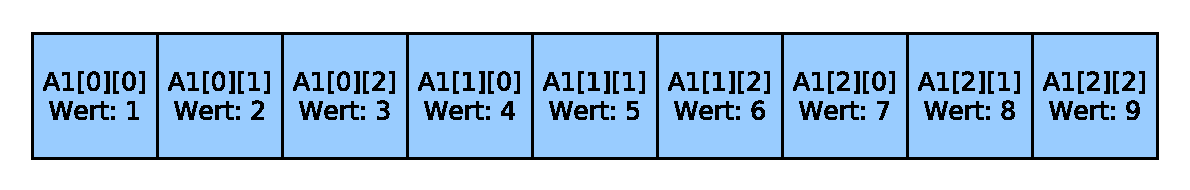
\includegraphics[width=\textwidth]{graphics/2darray_im_speicher}
  \caption{\label{fig:2darray} Das zweidimensionale Array \texttt{A1} im Speicher.}
\end{figure}

Die Benutzung von Feldern wird in folgendem Beispiel illustriert:
\begin{myexampleprogram}{Beispiel: Berechnung des Mittelwerts und der Varianz}
  Die Berechnung des Mittelwerts einer Datenreihe ist ein gutes Beispiel für die Benutzung von Arrays.
  Nehmen wir an, wir haben die folgenden Daten gegeben:
\begin{lstlisting}
double data[] = {1.3, 2.4, 5.3, 2.4, 6.7, 3.5, 6.9, 1.3, 1.4, 4.5,
                 5.5, 5.3, 6.7, 2.1, 2.4, 3.3, 7.9, 0.3, 3.3, 1.5};
\end{lstlisting}
  und wir wollen den Mittelwert dieser Daten berechnen.
  Folgendes Program übernimmt diese Aufgabe:
\begin{lstlisting}
#include <stdio.h>

int main()
{
  const int size = 20;
  double data[] = {1.3, 2.4, 5.3, 2.4, 6.7, 3.5, 6.9, 1.3, 1.4, 4.5,
                   5.5, 5.3, 6.7, 2.1, 2.4, 3.3, 7.9, 0.3, 3.3, 1.5};

  // initialisiere mean zu 0
  double mean = 0.;
  for (int i = 0; i < size; i++)
    {
      mean += data[i];
    }
  mean /= (double)size;
  printf("Der Mittelwert ist %e\n", mean);
  return (0);
}
\end{lstlisting}
  Für die Varianz müssen wir auch noch die Quadrate aufsummieren.
  Wir modifizieren dafür die Schleife wie folgt:
\begin{lstlisting}
double mean = 0., xsq = 0.;
for (int i = 0; i < size; i++)
  {
    mean += data[i];
    xsq += data[i] * data[i];
  }
mean /= (double)size;
\end{lstlisting}
  Die Varianz können wir dann wie folgt berechnen und ausgeben:
\begin{lstlisting}
double var = xsq / (double)size - mean * mean;
printf("Die Varianz ist %e\n", var);
\end{lstlisting}
\end{myexampleprogram}
\newpage

\subsection{Zeichenketten oder Strings}

In C gibt es keinen elementaren Datentyp für Zeichenketten, sogenannte \emph{strings}.
Zeichenketten werden mit Hilfe von Arrays abgebildet.
Ein Zeichen kann in einer Variablen vom Typ \verb|char| gespeichert werden.
Die Größe des Datentyps \texttt{char} ist immer ein Byte, also 8 Bit.\footnote{\textbf{Bemerkung:}~ Im ASCII Zeichensatz können $2^8= 256$ verschiedene Zeichen gespeichert werden.
Dies reicht für Englisch und ein paar Steuerzeichen, jedoch nicht für alle Sprachen dieser Welt.
Der ASCII Zeichensatz nutzt die ersten 128 Zustände (also die ersten 7 Bit) für das im Englischen genutzte Alphabet.
Die restlichen 128 Zustände werden abhängig vom  \emph{Encoding} interpretiert.
Für Deutsch kann man \texttt{latin-1} nutzen.
Je nach Encoding wird, z.B., ein Zeichen mit Wert 204 als solches oder jenes interpretiert.
Ist das Encoding nicht das richtige, erscheinen z.B. Zeichen mit Umlauten
nicht korrekt und scheinbar willkürliche Zeichen stehen an ihrer Stelle.
Sprachen, die mehr als 128 verschiedene Zeichen benötigen, können im oberen
Teil von ASCII überhaupt nicht dargestellt werden. Die Einsicht, dass es
mehr als 256 verschiedene Zeichen gibt, wurde im Unicode Standard
manifestiert. Die Konsequenz ist jedoch, dass jetzt mehr als ein Byte pro
Zeichen benötigt wird. UTF-8 ist inzwischen vielerorts das Standard-Encoding, sodass
beliebig viele verschiedene Zeichen in einer Textdatei genutzt werden
können. Der Preis ist jedoch, dass ein Buchstabe jetzt beliebig viele Byte
(meist eins) nutzt. Da hier der Fokus allerdings auf Numerischen Methoden
liegt, wird nicht weiter auf die vielfältigen Probleme mit Encodings
eingegangen.}

Eine Zeichenkette kann also durch eine Array von Elementen vom Typ \verb|char| erzeugt werden.
Das Ende einer Zeichenkette wird durch das Zeichen \verb|\0| angegeben.
Man spricht auch von \emph{null-terminiert} oder \emph{0-terminiert} und das Zeichen \verb|\0| wird auch \emph{Nullterminierungszeichen} genannt.
Im nächsten Beispiel überprüfen wir, ob eine Zeichenkette eine Zahl enthält:
\begin{myexampleprogram}{Beispiel: Durchsuchen von Zeichenketten}
\begin{lstlisting}
#include <stdio.h>

int main()
{
  char string[] = "sdfk99225kljsdfs\0";
  int i = 0;
  int ergebnis = 0;

  while(1) {
    if(string[i] == '\0') {
      break;
    }
    if((string[i]) >= '0' && (string[i] <= '9')) {
      ergebnis = 1;
      break;
    }
    i++;
  }
  if (ergebnis){
    printf("Der String %s enthaelt mindestens eine Zahl\n", string);
  } else {
    printf("Der String %s enthaelt keine Zahlen\n", string);
  }
  return 0;
}
\end{lstlisting}
\end{myexampleprogram}
Wir deklarieren und initialisieren zunächst die Variable \texttt{string} mit einer Zeichenkette.
Dann nutzen wir eine \verb|while| Schleife mit konstant wahrem logischem Ausdruck.
Die Schleife wird dann mit \verb|break| abgebrochen, wenn das Endstring-Zeichen gefunden wurde.
In der Schleife wird dann jedes Element der Kette darauf überprüft, ob es eine Zahl ist.
Dementsprechend wird die Variable \verb|ergebnis| gesetzt.
% BaKo: hier m.E. keine gute Stelle, um darauf hinzuweisen
%       erstens sind Strings speziell (weil terminiert)
%       zweitens sind die *printf Funktionen schrecklich kompliziert...
% Beim abschließenden \texttt{printf} wird eine wichtige Eigenschaft von \texttt{C} Feldern deutlich:
% Man benötigt keine Referenzierungsoperator \verb|&|.\index{Adressoperator \&}\index{\&}
% Im nächsten Abschnitt über Zeiger wird klar werden, warum dies so ist.

\subsubsection{Formatierte Erstellung von Zeichenketten mit \texttt{sprintf} und \texttt{snprintf}}

Die Manipulation von Zeichenketten ist oft ein wichtiger Bestandteil eines Programms, zum Beispiel um Ausgabedateinamen abhängig vom Wert einer Variable zu machen.

Wie haben die Funktion \texttt{printf} schon öfter zur Textausgabe verwendet und werden im Detail in Teil~\ref{sec:ein_ausgabe} auf die \emph{formatierte} Ausgabe eingehen.
Möchte man jedoch formatierte Textdarstellungen von Variablen nicht auf die Konsole, sondern direkt in eine Zeichenkette ausgeben, so stehen in \texttt{C} die beiden Funktionen \texttt{sprintf} und \texttt{snprintf} zur Verfügung.
Diese ähneln in ihrer Benutzung der bekannten \texttt{printf} Funktion und werden mit der Headerdatei \texttt{stdio.h} eingebunden.\index{\texttt{sprintf}}\index{\texttt{snprintf}}
Im Gegensatz zu \texttt{printf}, schreiben diese Funktionen jedoch direkt in eine sich im Speicher befindliche Zeichenkette.

Diese Funktionen haben die Signaturen
\begin{lstlisting}
  int sprintf(char *str, const char *format, ...);
  int snprintf(char *str, size_t size, const char *format, ...);
\end{lstlisting}
wobei das Argument \enquote{\texttt{str}} für die Zeichenkette steht, in die geschrieben werden soll und \enquote{\texttt{format}} eine konstante Zeichenkette ist, in der wir beschreiben werden, wie dies zu erfolgen hat.
Die Bedeutung von \enquote{\texttt{char *}} und \enquote{\texttt{const char *}} wird in Teil~\ref{sec:zeiger} noch genau erklärt werden.
Die sogenannte \emph{variable Argumentenliste}, \enquote{\texttt{...}}, dient bei den Funktionen aus \texttt{stdio.h} als Platzhalter für eine beliebige Anzahl von Variablen oder Konstanten, die man ausgeben möchte.
Bei \texttt{snprintf} steht das Argument \enquote{\texttt{size}} für die maximale Anzahl an Zeichen (inklusive des Nullterminierungszeichens), welche in die Zeichenkette \texttt{str} geschrieben werden soll.
Die Stelle in der Zeichenkette, an denen diese Ausgabe stattfinden soll, sowie das Format in der diese Ausgabe erfolgen soll, geben wir anhand von Platzhaltern an, genau so, wie wir es auch schon bei \texttt{printf} getan haben.

Da wir jedoch nicht auf die Konsole ausgeben, sondern direkt in Speicher schreiben, muss man bei der Verwendung insbesondere von \texttt{sprintf} sehr vorsichtig sein, wie in folgendem Beispiel gezeigt wird.

\begin{myexampleprogram}{Beispiel: Formatierte Erstellung von Zeichenketten mit \texttt{sprintf} und \texttt{snprintf}}
\begin{lstlisting}[numbers=left]
#include <stdio.h>
// konstante Längen für lange und kurze Zeichenketten
const int MAX_LENGTH = 1000;
const int SHORT_LENGTH = 50;

int main()
{
  char string[MAX_LENGTH];
  const int i = 42;
  sprintf(string,
          "The Answer to the Ultimate Question of Life,"
          "The Universe, and Everything is %d.\n\n",
          i);
  printf("string: %s", string);
  
  int rval;
  char short_string[SHORT_LENGTH];
  
  // kurze Zeichenkette wird in short_string geschrieben
  // Rueckgaberwert wird ueberprueft
  rval = snprintf(short_string, 
                  SHORT_LENGTH-1, 
                  "This is a test string.\n\n");
  if(rval >= SHORT_LENGTH) {
    printf("snprintf: The string was not completely written!\n");
  } else {
    printf("snprintf: wrote %d characters\n", rval);
  }
  printf("short_string: %s",short_string);
  
  // ueberlange Zeichenkette wird in short_string geschrieben
  // Rueckgaberwert wird ueberprueft
  rval = snprintf(short_string, 
                  SHORT_LENGTH-1, 
                  "The Answer to the Ultimate Question of Life, "
                  "The Universe, and Everything is %d.\n", 
                  i);
                  
  if(rval >= SHORT_LENGTH) {
    printf("snprintf: The string was not completely written!\n");
  }
  
  printf("short_string: %s\n\n",short_string);
  
  // ACHTUNG: hier wird fremder Speicher ueberschrieben 
  sprintf(short_string, 
          "The Answer to the Ultimate Question of Life"
          ", The Universe, and Everything is %d.\n",
          i);
  printf("short_string: %s",short_string); 
  
  return 0;
}
\end{lstlisting}
\noindent \textbf{Ausgabe des Beispielprogramms:}
{\footnotesize
\begin{lstlisting}[numbers=left]
$ ./test
string: The Answer to the Ultimate Question of Life, The Universe, and Everything is 42.

snprintf: wrote 24 characters
short_string: This is a test string.

snprintf: The string was not completely written!
short_string: The Answer to the Ultimate Question of Life, The

short_string: The Answer to the Ultimate Question of Life, The Universe, and Everything is 42.
\end{lstlisting}
}

\end{myexampleprogram}
Ebenso wie bei \texttt{scanf}, besteht die Gefahr eines buffer overflows, wenn mit \texttt{sprintf} mehr Zeichen geschrieben werden, als eigentlich allokiert wurden.
Dies resultiert im schlimmsten Fall \emph{nicht} in einem Programmabsturz sondern darin, dass irgendeine Speicherstelle überschrieben wird.

Es ist deshalb Vorsicht geboten und \texttt{snprintf} sollte \texttt{sprintf} vorgezogen werden, da erstere Funktion es erlaubt, die Länge der geschriebenen Zeichenkette zu beschränken.
Desweiteren kann man durch Überprüfung des Rückgabewertes der Funktion feststellen, ob die Zeichenkette in den vorhandenen Speicher gepasst hat und so direkt auf mögliche Fehler reagieren.
Wie man an der folgenden Ausgabe sehen kann, schreibt das Programm in der Anweisung in den Zeilen $46$ bis $49$ in fremden Speicher.
\texttt{printf} liest bei Angabe von \texttt{\%s} die angegebene Speicherstelle immer bis zum nächsten Nullterminierungszeichen aus.

\begin{myalertblock}{Anmerkung: konstante Zeichenketten teilen}
Im vorherigen Beispiel haben wir uns der Eigenschaft konstanter Zeichenketten in \texttt{C} bedient, dass mehrere, aufeinander folgende und nicht mit Kommata getrennte Zeichenketten zu einer einzigen Zeichenkette Zusammengefasst werden.
Der Compiler interpretiert
\begin{lstlisting}
  "Zeichenkette mit Platzhalter: %d "
  "Zweite Zeichenkette"
\end{lstlisting}
also als
\begin{lstlisting}
  "Zeichenkette mit Platzhalter: %d Zweite Zeichenkette"
\end{lstlisting}
was es uns erlaubt, den Quelltext für das Beispielprogramm durch Zeilenumbrüche sauberer und verständlicher zu gestalten.
\end{myalertblock}

\endinput

\section{Die Bibliotheken \texttt{math.h} und \texttt{complex.h}}

Die Sprache \texttt{C} hat neben den Sprachbestandteilen auch eine umfangreiche Liste von Standardbibliotheken.
Sie sind im \texttt{ANSI C} Standard festgelegt.
Diejenige für die Ein- und Ausgabe haben wir schon kennengelernt.
Wir werden jetzt noch zwei weitere kurz einführen.

\subsection{Mathematische Bibliothek \texttt{math.h}}

Erstens die Bibliothek \texttt{math.h}.
Sie stellt mathematische Funktionen, wie beispielsweise trigonometrische Funktionen, aber auch eine Funktion für den Betrag zur Verfügung.
Natürlich berechnen diese Funktionen das Ergebnis nur zur gewünschten Genauigkeit.
Wir illustrieren dies am Bespiel vom Cosinus.
Die Cosinus Funktion ist auf ganz $\mathbb{R}$ durch eine Taylorreihe um 0 definiert.
\begin{equation}
  \label{eq:cos}
  \cos\left(x\right)\ =\ \sum_{l=0}^{\infty} \left(-1\right)^{l} \dfrac{x^{2l}}{\left(2l\right)!}\,.
\end{equation}
Die Funktion 
\begin{lstlisting}
  double cos(double x);
\end{lstlisting}
berechnet den Cosinus in \texttt{double} Genauigkeit.
Im folgenden Quelltext berechnen wir den Cosinus einmal mit Hilfe der Funktion aus \texttt{math.h} und einmal über die Reihenentwicklung, die wir zu einer angegebenen Ordnung abbrechen:
\begin{lstlisting}[caption={Beispiel zur Verwendung des Cosinus}, belowcaptionskip=0.3em]
#include <math.h>
#include <stdio.h>
#include <stdlib.h>

int main(int argc, char *argv[])
{
  double winkel;
  double coswinkel;
  // genuegend Kommandozeilenparameter?
  if (argc < 2) {
    printf("Usage: ./print_cos Winkel Naeherungsordnung[optional]\n");
    return(-1);
  }
  winkel = atof(argv[1]);  // Konvertiert eine Zeichenkette in eine Fliesskommazahl
  coswinkel = cos(winkel); // cos aus math.h
  printf("Winkel=%e \t cos(Winkel) = %e\n", winkel, coswinkel);
  // nun selbst, wenn die Naeherungsordnung gegeben wurde
  if (argc > 2) {
    int n;
    double coswinkelapprox;
    double zaehler = winkel; // Zaehler
    int nenner = 1;          // Nenner
    n = atoi(argv[2]);       // atoi konvertiert eine Zeichenkette in eine ganze Zahl
    coswinkelapprox = 1.;    // Das Ergebnis zu fuehrender Ordnung
    for (int i = 1; i < n; ++i) {
      int sign = 1;          // (-1)^l ist entweder 1 oder -1, wenn l gerade
      if( (i % 2) == 1 ) sign = -1; // oder ungerade ist
      zaehler = zaehler * zaehler;
      nenner = nenner * (2 * i - 1) * 2 * i;
      coswinkelapprox += sign * zaehler / nenner;
    }
    printf("cos(Winkel) approx %e\n", coswinkelapprox);
  }
  return(0);
}
\end{lstlisting}
Wenn auf der Kommandozeile die Ordnung der Näherung als zweiter Kommandozeilenparameter angegeben wurde, berechnen wir auch die Näherung selbst nach der Formel Gleichung~\ref{eq:cos}.
Wie schon vorher erklärt, sind die Kommandozeilenparameter in der \texttt{main} Funktion nur als Zeichenkette verfügbar.
Die Konvertierung der Ordnung in eine ganze Zahl kann man mit der standard Funktion \texttt{atoi} (ASCII to integer) durchführen.
Genauso verwenden wir \texttt{atof} (ASCII to float) um den eingegebenen Winkel in the Fließkommazahl umzuwandeln.
Man beachte, dass die standard Cosinus Funktion das Argument im Bogenmaß erwartet.

Bei der Berechnung der Näherung müssen wir nicht in jedem Schritt die Potenz $x^{2i}$ und Fakultät $(2i)!$ neu berechnen, sonder müssen lediglich die Variablen \texttt{zaehler, nenner} entsprechend auffrischen.
Dies ist ein generelles Konzept: Man verwendet mehr Speicher um Rechnung zu sparen.

\subsubsection{Übersetzen und Linken mit \texttt{math.h}}

Das Programm kann man wie folgt übersetzen

\vspace*{0.5cm}
\begin{verbatim}
>$  gcc -std=c99 -Wall -pedantic cosineexample.c -o cos.exe -lm
\end{verbatim}
\vspace*{0.5cm}

\noindent Man beachte, dass man nun explizit die Bibliothek \texttt{math.h} dazulinken muss.
Dies geschieht mit dem Argument \texttt{-lm}.
In Tabelle~\ref{math} listen wir einige wichtige Funktionen auf, die \texttt{math.h} bereitstellt.

\begin{table}[t]
  \centering
  % centering table
  \begin{tabular}{|l l|}
    \hline
    \texttt{Deklaration} & \texttt{Rückgabewert} \\
    % creating 10 columns
    \hline
    \texttt{double acos(double x);} & Arcuscosinus von \texttt{x}\\
    \texttt{double asin(double x);} & Arcussinus von \texttt{x}\\
    \texttt{double atan(double x);} & Arcustangenz von \texttt{x}\\
    \texttt{double atan2(double y,double x);} & Arcustangenz von \texttt{x/y}\\
    \texttt{double ceil(double x);} & Kleinste ganze Zahl, welche $\ge$ \texttt{x} ist \\
    \texttt{double cos(double x);} & Cosinus von \texttt{x}\\
    \texttt{double cosh(double x);} & Cosinus hyperbolicus von \texttt{x}\\
    \texttt{double exp(double x);} & $e^{x}$ wobei $e=2.7182..$\\
    \texttt{double fabs(double x);} & $\vert x\vert$\\
    \texttt{double floor(double x);} & Größte ganze Zahl, welche $\le$ \texttt{x} ist \\
    \texttt{double ldexp(double x, double y);} & $xe^{y}$ \\
    \texttt{double log(double x);} & Natürlicher Logarithmus von \texttt{x}\\
    \texttt{double log10(double x);} & Zehnerlogarithmus von \texttt{x}\\
    \texttt{double pow(double x, double y);} & $x^{y}$\\
    \texttt{double sin(double x);} & Sinus von \texttt{x}\\
    \texttt{double sinh(double x);} & Sinus hyperbolicus von \texttt{x}\\
    \texttt{double sqrt(double x);} & $\sqrt{x}$\\
    \texttt{double tan(double x);} & Tangens von \texttt{x}\\
    \texttt{double tanh(double x);} & Tangens hyperbolikus von \texttt{x}\\
    \hline
  \end{tabular}
  \caption{Einige Funktionen, die in \texttt{math.h} deklariert sind.\label{math}}
\end{table}

\subsection{Komplexe Zahlen mit \texttt{complex.h}}

Als zweite Standardbibliothek weisen wir noch auf \texttt{complex.h} hin.\index{\texttt{complex.h}}
Sie stellt einen komplexen Datentyp zur Verfügung, der leider nicht Teil von C selbst ist.
Die Benutzung ist dann aber gleich zu \texttt{C} Datentypen, wie man an folgendem Beispiel sieht:\index{\texttt{I}}\index{\texttt{complex}}\index{\texttt{cexp}}\index{Datentypen!\texttt{complex}}\index{Datentypen!\texttt{double complex}}
\begin{lstlisting}[caption={Beispiel für komplexe Zahlen}, belowcaptionskip=0.3em]
  #include <stdlib.h>
  #include <stdio.h>
  #include <math.h>
  #include <complex.h>
  
  int main(int argc, char *argv[])
  {
    double complex z,v,w;

    // I ist die rein komplexe Zahl i
    z = 1 + I*3;
    v = 0.3*I;
    // komplexe Multiplikation
    w = z*v;
    // Zugriff auf Real- und Imaginaerteile
    printf(``w = %e + i*%e\n'', creal(w), cimag(w));
    // Anwendung der komplexen Exponetialfunktion
    z = cexp(w);
    printf(``w = %e + i*%e\n'', creal(z), cimag(z));
    return 0;
  }
\end{lstlisting}

\subsubsection{Mathematische Funktionen für komplexe Zahlen}

In \texttt{math.h} sind wiederum die Funktionen aus Tabelle~\ref{math} für den Typ \texttt{double complex} definiert.\index{\texttt{math.h}}
Meistens unterscheiden sie sich von den reellwertigen Funktionen nur duch ein vorgestelltes \texttt{'c'}, wie zum Beispiel bei \texttt{cexp}.\index{\texttt{cexp}}
Auf Real- und Imaginärteil kann mit \texttt{creal} und \texttt{cimag} zugegriffen werden.
\texttt{complex.h} stellt auch Typen \texttt{float complex} und \texttt{long double complex} bereit.
Die entsprechenden Exponentialfunktionen heißen dann \texttt{cexpf} und \texttt{cexpl}.
Das komplex konjugierte erhält man mit \texttt{conj}, bzw. \texttt{conjf} und \texttt{conjl}.
\index{\texttt{complex.h}}\index{\texttt{creal}}\index{\texttt{cimag}}\index{\texttt{conj}}

\chapter{Zeiger und Co}
Im folgenden Kapitel werden zum Abschluss noch die beiden wichtigen Themen Zeiger und die damit verbundene dynamische Speicherverwaltung und zusammengesetzte Datentypen eingeführt.
Dabei handelt es sich um etwas fortgeschrittenere Konzepte, die aber auch die wahre Stärke von \texttt{C} ausmachen.
Mit Hilfe von Zeigern wird auch eine Implementierung vom Algorithmus \emph{Einfügesortieren} gegeben.

\section{Zeiger}\label{sec:zeiger}

Kommen wir nun zu der Frage, wie man aus Funktionen mehr als nur skalare Größen zurück gibt.
Genauso, wie wir Felder an Funktionen uebergeben können, wollen wir auch Felder als Rückgabewert benutzen.
Dies geht in \texttt{C} nicht direkt, sondern nur über den Umweg von sogenannten Zeigern.
Zeiger sind mit das mächtigste Sprachelement in \texttt{C}.
Sie sind allerdings auch für jede Menge Verwirrung und Programmierfehler verantworlich.
\index{Zeiger}

\begin{figure}[h]
  \centering
  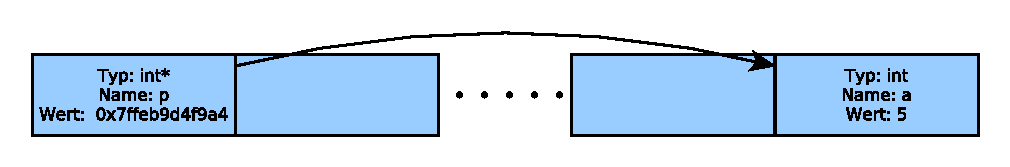
\includegraphics[width=\linewidth]{graphics/zeiger}
  \caption{\label{fig:zeiger} Illustration Zeiger.}
\end{figure}

Um Zeiger verstehen zu können, muss man sich zunächst klar machen, dass eine Variable im Prinzip aus zwei Dingen besteht:
Einerseits dem Typ der Variablen und andererseits der Speicheradresse, unter der ihr Wert abgelegt wird.
Über den Typ der Variablen weiß der Compiler, wie viele Bits im Speicher belegt sind, und wenn die Anfangsadresse für das erste Bit bekannt ist, dann kann die gesamte Anzahl an Bits ausgelesen und dem Typ entsprechend interpretiert werden.
\texttt{C} erlaubt Zugriff sowohl auf den Wert einer Variablen, als auch auf die Adresse, an der der Wert abgelegt ist.
Unterschieden wird zwischen den beiden mit dem \verb|&| Operator.
Für eine Variable \verb|n| repräsentiert \verb|n| den Wert und \verb|&n| die Speicheradresse.
Bei \verb|&n| spricht man auch von Zeiger (\emph{pointer}) und bei \verb|&| vom Adressoperator.\index{Adressoperator \&}\index{\&}
Mit Hilfe von \texttt{printf} kann man den Unterschied ausgeben

\begin{minipage}{\linewidth}
\begin{lstlisting}
  int a = 5;
  int * p = &a;
  printf("Der Wert %d ist an der Adresse %p abgelegt.\n", a, p);
\end{lstlisting}
\end{minipage}
was eine Ausgabe wie die folgende erzeugt
\begin{verbatim}
  Der Wert 5 ist an der Adresse 0x7ffeb9d4f9a4 abgelegt.
\end{verbatim}
Die Adresse wird hier als \emph{Hexadezimalzahl} \verb|0x7ffeb9d4f9a4| ausgegeben.
Die Beziehung von \verb|p| und \verb|a| ist in Abbildung~\ref{fig:zeiger} illustriert.

Da Zeiger in \texttt{C} eine sehr wichtige Rolle spielen, gibt es für sie spezielle Datentypen, wie im letzten Beispiel schon gesehen:

\begin{minipage}{\linewidth}
\begin{lstlisting}
int n = 3; // eine Variable vom Typ int
int *address; // eine Variable vom Typ Zeiger auf int
address = &n; // address zeigt auf n
*address = 5; // *address representiert den Wert, der unter der Adresse address
              // gespeichert ist. man spricht von dereferenzieren
n == 5; // ist jetzt wahr.
\end{lstlisting}
\end{minipage}
Genauso gibt es einen Typ Zeiger auf \verb|double|, nämlich \verb|double*| und so weiter.
Allgemein ist ein Zeiger eine Variable, die eine Adresse als Wert zusammen mit einem Datentyp speichert.
Wir demonstrieren die Nützlichkeit von Zeigern zunächst an einem Beispiel.
Wir definieren eine Funktion, die zwei Parameter \verb|a, b| übergeben bekommt und diese jeweils um eins erhöht.
Anschließend sollen diese beiden neuen Werte zurückgegeben werden.

Ein Weg, um dies zu tun, ist das sogenannte \emph{call by reference}.
\index{call by reference}
Was \textbf{nicht} funktioniert ist das folgende:

\begin{minipage}{\linewidth}
\begin{lstlisting}
#include <stdio.h>
// einfache Funktion um a,b um 1 zu erhoehen
void increment(int a, int b)
{
  a++;
  b++;
  return;
}

int main()
{
  int a = 2, b = 3;
  printf("Wert vor der Funktion a=%d, b=%d\n", a, b);
  increment(a, b); // die Variablen in unserem Block werden
                         // nicht veraendert!
  printf("Wert nach der Funktion a=%d, b=%d\n", a, b);
  return 0;
}
\end{lstlisting}
\end{minipage}

Der Grund ist, dass in der Funktion \verb|increment| neue Variablen \verb|a|, \verb|b| angelegt werden, die nur in der Funktion selbst sichtbar sind.
Sie haben also nichts mit den Variablen \verb|a|, \verb|b| in der Funktion \verb|main| gemein, außer dem Namen.
Man spricht hier von \emph{call by value}, da die Variablen \verb|a, b| in der Funktion \verb|increment| mit den Werten der Variablen aus \verb|main| initialisiert werden.\index{call by value}
Deswegen liefern die \verb|printf| Aufrufe in den Zeilen 12 und 15 das gleiche Ergebnis.
Denn die Variablen \verb|a|, \verb|b| in \verb|main| wurden nicht verändert.

Bei \emph{call by reference} wird an Stelle des Wertes die Adresse übergeben.\index{call by reference}

\begin{minipage}{\linewidth}
\begin{lstlisting}
#include <stdio.h>
// einfache Funktion um a,b um 1 zu erhoehen
void increment(int *a, int *b)
{
  (*a)++;
  (*b)++;
  return;
}

int main()
{
  int a = 2, b = 3;
  printf("Wert vor der Funktion a=%d, b=%d\n", a, b);
  increment(&a, &b); // die Variablen in unserem Block werden
                           // direkt veraendert!
  printf("Wert nach der Funktion a=%d, b=%d\n", a, b);
  return 0;
}
\end{lstlisting}
\end{minipage}
Die Funktion bekommt also zwei Parameter vom Typ \verb|int*|, also Zeiger auf \verb|int|.
Dann wird mit dem Dereferenzierungsoperator \verb|*| der Wert, der unter den beiden Adressen gespeichert ist, um eins erhöht.
Das geschieht unter der Annahme, dass dort eine Variable vom Typ \verb|int| abgelegt ist.
Damit werden also direkt die Werte der Variable \verb|a, b| in \verb|main| verändert.

Zeiger kann man genau wie andere Variablen nutzen (womit auch klar ist, dass man auch Zeiger auf Zeiger definieren kann).
Folgendes Beispiel illustriert die Nutzung noch einmal, wobei \verb|NULL| der Nullzeiger ist, welcher auf eine reservierte Adresse zeigt, die nicht dereferenziert werden kann:\index{\texttt{NULL}}

\begin{minipage}{\linewidth}
\begin{lstlisting}[numbers=left]
#include <stdio.h>

int main()
{
  int q = 10;
  int *p = NULL;
  p = &q;
  printf("Der Wert an der Adresse %p ist:%d\n", p, *p);
  return 0;
}
\end{lstlisting}
\end{minipage}

In der fünften Zeile haben wir eine Variable vom Typ \verb|int| deklariert und mit dem Wert 10 initialisiert, in der sechsten Zeile eine Variable vom Typ \verb|int*|, die mit dem \verb|NULL| Zeiger initialisiert wurde.
In der siebten Zeile wird dann \verb|p| auf die Adresse von \verb|q| gesetzt.
Damit liefert die Dereferenzierung von \verb|p|, also \verb|*p|, den Wert von \verb|q|.
Zeigern dürfen nur gültige Adressen zugewiesen werden.
Dies kann allerdings, bis auf Ausnahmen, nicht vom Compiler überprüft werden.
Wenn doch keine gültige Adresse zugewiesen wurde, bekommt man bei Dereferenzierung den \emph{segmentation fault} als Laufzeitfehler.\index{segmentation fault}
Dieser Quelltext weist sehr wahrscheinlich eine ungültige Adresse zu:
\begin{lstlisting}
int *p = 42;
\end{lstlisting}
Allerdings wird in diesem Fall der Compiler sehr wahrscheinlich\footnote{Hängt leider vom Compiler ab.} eine Warnung geben, denn 42 ist vom Typ \verb|int|, und nicht vom Typ \verb|int*|.
GCC 6.3.1 gibt folgendes aus:
\begin{verbatim}
int-ptr.c:7:14: Warnung: Initialisierung erzeugt Zeiger 
           von Ganzzahl ohne Typkonvertierung [-Wint-conversion]
     int *p = 42;
              ^~
\end{verbatim}
Wenn der Compiler sich hier nicht beschwert, sollte man die Dokumentation studieren, um heraus zu finden, wie man diesen Typ von Warnung anschalten kann, oder, wenn das nicht möglich ist, den Compiler wechseln.

\subsection{Zeiger und Felder}

\index{Feld}\index{array}
Wie schon im Abschnitt über Felder angedeutet sind Felder und Zeiger in \texttt{C} eng verwandt.
Nehmen wir an, es wurde ein Feld wie oben eingeführt deklariert
\begin{lstlisting}
  int n[] = {1, 2, 3, 4, 5};
\end{lstlisting}
Dann ist die Variable \verb|n| eng verwandt mit dem Typ \verb|int *|, also Zeiger auf \verb|int|.
Den subtilen Unterschied kann man am ehesten damit erklären, dass \verb|n| konstant ist, also die Adresse nicht verändert werden darf.
Das bedeutet, dass folgender \texttt{C} Quelltext korrekt ist
\begin{lstlisting}
  int n[] = {1, 2, 3, 4, 5};
  int * p = n;
\end{lstlisting}
und auch die folgenden zwei Funktionsdeklarationen äquivalent sind
\begin{lstlisting}
  void f1(int * a, const int n);
  void f2(int a[], const int n);
\end{lstlisting}
Daraus folgt auch, dass ein Feld in \texttt{C} immer \emph{by reference} übergeben wird.\index{call by reference}
Wird in Funktion \texttt{f1} oder \texttt{f2} in das Feld \texttt{a} geschrieben, so wird das ursprüngliche Feld aus dem aufrufenden Quelltextblock modifiziert.
Obiges Beispiel kann man also auch wie folgt schreiben:
\begin{lstlisting}
  #include <stdio.h>
// einfache Funktion um a,b um 1 zu erhoehen
void increment(int *a, const int n)
{
  for(int i = 0; i < n; i++) {
    a[i]++;
  }
  return;
}

int main()
{
  int a[] = {2, 3};
  printf("Wert vor der Funktion a[0]=%d, a[1]=%d\n", a[0], a[1]);
  increment(a, 2); // die Variablen in unserem Block werden
                           // direkt veraendert!
  printf("Wert nach der Funktion a[0]=%d, a[1]=%d\n", a[0], a[1]);
  return 0;
}
\end{lstlisting}
Wenn das übergebene Feld innerhalb einer Funktion nicht verändert werden soll, so kann man es als \verb|const| deklarieren \index{\texttt{const}}
\begin{lstlisting}
  void f(const int * a, const int n);
\end{lstlisting}

Als etwas ausführlicheres Beispiel für die Verwendung von Feldern, dient uns folgende numerische Abschätzung der Zahl $\pi$:
\begin{myexampleprogram}{Beispiel: \texttt{Näherung von $\pi$}}
  In diesem Beispiel berechnen wir $\pi$ näherungsweise.
  Dafür verwenden wir folgende Integraldarstellung von $\pi$:
  \begin{equation}
    \pi=4\cdot \int_{0}^{1} \mathrm{d}x \dfrac{1}{1+x^2}
  \end{equation}
  Das Integral berechnen wir numerisch, indem wir die Fläche unterhalb der Kurve als eine Summe abschätzen.
  Dabei bedienen wir uns der sogenannten Trapez-Regel.
  Wir teilen das Interval $[0,1]$ in $N$ gleichlange Unterintervalle auf.
  Den jeweilige linke Punkt des Intervals nennen wir $x_i$, $i=0,...,N$, wobei $x_n-x_{n-1}=\Delta=\mathrm{const}$.
  Auf jedem Unterintervall approximieren wir die Funktion linear, wie in folgender Abbildung dargestellt ist:
  \begin{center}
    %\begin{minipage}
    \includegraphics[width=.6\linewidth]{trapez1}
  \end{center}
  In unserem Fall sind die Punkte wie folgt gegeben
  \begin{displaymath}
    x_i = i/N\,,\qquad i = 0, ..., N-1\,.
  \end{displaymath}
  Definieren wir folgende Funktion
  \[
  f(x) = \frac{1}{1+x^2}\,,
  \]
  so können wir wie folgt über die Teilergebnisse summieren:
  \begin{equation}
    \int_{0}^{1} \mathrm{d}x \dfrac{1}{1+x^2}\approx \sum_{i=0}^{N-1}\frac{1}{2N}[f(x_i)+f(x_{i+1})]
  \end{equation}
  Hier ist der entsprechende \texttt{C} Quelltext, der Arrays benutzt:
\begin{lstlisting}[numbers=left]
#include <stdio.h>
const int MAX = 10000;

int main()
{
  int N = 0;
  double f[MAX], x[MAX]; // double arrays der Laenge MAX
  scanf("%d", &N);
  // Pruefe die Eingabe
  if (N >= MAX)
    {
      printf("Fehler, zu vielen Stuetzstellen\n");
      return (-1);
    }
  if (N < 0)
    {
      printf("N muss groesser als 0 sein!\n");
      return (-2);
    }
  for (int i = 0; i < N; ++i)
    {
      x[i] = (double)i / (double)N;
      f[i] = 1. / (1 + x[i] * x[i]);
    }
  double summe = 0.;
  for (int i = 0; i < N - 1; ++i)
    {
      summe += (f[i] + f[i + 1]);
    }
  summe += f[N - 1] + 0.5; // Randterm
  printf("Die Naeherung von pi ist =%e\n", 2. / N * summe);
  return (0);
}
\end{lstlisting}
  Neben der Benutzung von Arrays, haben wir noch ein weiteres neues Konzept eingeführt.
  Bei der Division von $i/N$, beide vom Typ \verb|int|, in Zeile $22$ haben wir einen expliziten \emph{cast} nach \verb|double| durchgeführt, damit keine Division ganzer Zahlen durchgeführt wird.

  Dieses Beispiel hätten wir natürlich auch ohne Arrays durchführen können, aber es illustriert deren Benutzung.
\end{myexampleprogram}

\subsection{Die Parameter der \texttt{main} Funktion} \label{subsec:CommandLineArguments}

\index{\texttt{argc}}
\index{\texttt{argv}}

An dieser Stelle können wir jetzt auch die möglichen Parameter der Funktion \verb|main| einführen.
Die ist nämlich allgemein wie folgt deklariert:\index{\texttt{argc}}\index{\texttt{argv}}\index{\texttt{main}}
\begin{lstlisting}
int main(int argc, char *argv[]);
\end{lstlisting}
An der Kommandozeile kann man mit Hilfe der Funktionsargumente von \verb|main| dem Programm Parameter übergeben.
Die Funktion \verb|main| erhält diese in Form einer Zeichkette.
Leerzeichen in dieser Zeichenkette werden als Trennzeichen interpretiert, so dass die Zeichenkette \verb|argc| Wörter enthält.
Das erste Wort ist immer der Name der Programms.
Die Wörter werden in \verb|argv| gespeichert.
Also, zum Bespiel
\begin{verbatim}
  ./main.exe 3 hallo
\end{verbatim}
liefert 
\begin{itemize}
\item \verb|argc=3|
\item \verb|argv[0] = "./main.exe"|
\item \verb|argv[1] = "3"|
\item \verb|argv[2] = "hallo"|
\end{itemize}

\subsection{Zeigerarithmetik}

Man kann auch eine Zeichenkette initialisieren:
\begin{lstlisting}
#include <stdio.h>
int main()
{
  char string[] = {'H', 'e', 'l', 'l', 'o', ' ', 'w', 'o', 'r', 'l', 'd', '\0'};
  char *pointer = NULL;
  pointer = &string[6];
  printf("Das siebte Zeichen im String ist %c\n", *pointer);
  return (0);
}
\end{lstlisting}
und dann mit \verb|pointer| auf einzelne Elemente der Zeichenkette zugreifen.
Das ist nicht nur ein alternativer Weg, um auf die Elemente eines Arrays zuzugreifen.
\texttt{C} stellt Zeiger intern als ganze Zahlen dar und auf jedem Zeigertyp sind auch arithmetische Operationen definiert.
Beispielsweise ist folgendes in \texttt{C} korrekter Quelltext:
\begin{lstlisting}
int list[5];
int *plist = NULL;
plist = list; // aequivalent zu plist = &list[0];
for (int i = 0; i < 5; i++)
  {
    *plist = i;
    plist++; // aequivalent zu plist = plist + 1; oder plist += 1;
  }
\end{lstlisting}
Mit unserer bisherigen Kenntnis des Operators \verb|++| würden wir erwarten, dass der Wert von \verb|plist| um eins erhöht wird.\index{Zeiger!\texttt{++}}\index{Zeiger!\texttt{*}}
Das ist im Prinzip auch richtig, allerdings findet die Erhöhung in Einheiten der Länge des Typs, auf den der Zeiger zeigt.
Und damit zeigt \verb|plist++| auf das nächste Element in der Liste \verb|list|.
Denn \texttt{C} reserviert für \verb|int list[5];| einen zusammenhängenden Speicherbereich der fünffachen Länge von \verb|int|.
\verb|list|, ohne den Indexoperator, ist selbst vom Typ \verb|int*|, und zeigt auf den Anfang dieses Speicherbereichs.
\verb|list[3]| ist dann äquivalent zu folgender Dereferenzierung: \verb|*(list + 3)|.
Und damit weißt obiger Beispielcode dem $i$ten Element von \verb|list| den Wert $i$ zu.
Genauso kann man den Indexoperator für Zeiger verwenden.
Im obigen Beispiel hätten wir auch
\begin{lstlisting}
int list[5];
int *plist = NULL;
plist = list; // equivalent zu plist = &list[0];
for (int i = 0; i < 5; i++)
  {
    plist[i] = i;
  }
\end{lstlisting}
schreiben können.
Im folgenden Beispiel finden sich einige der möglichen arithmetischen Operationen für Zeiger:
\begin{lstlisting}
#include <stdio.h>

int main()
{
  int sqnum[] = {1, 4, 9, 16, 25, 36, 49};
  int *pointer;
  int *pointer2;
  pointer = sqnum;
  pointer++;
  printf("Nach der Inkrementierung des Zeigers %d\n", *pointer);
  pointer--;
  printf("Nach der Dekrementierung des Zeigers %d\n", *pointer);
  pointer += 2;
  printf("Nach dem Hinzufuegen von 2 zum Zeiger %d\n", *pointer);
  pointer -= 2;
  printf("Nach dem Subtrahieren von 2 vom Zeiger %d\n", *pointer);
  ++pointer;
  pointer2 = &sqnum[4];
  printf("Zwischen pointer2 und pointer gibt es %ld Elemente\n",
         pointer2 - pointer);
  return (0);
}
\end{lstlisting}
Überlegen Sie sich, was obiges Programm als Ausgabe erzeugen wird, bevor Sie diesen Quelltext übersetzen und ausführen lassen.
%Die \verb|++| Operation auf einen Zeiger vom Typ \verb|int| ist in Abbildung~\ref{pointinc} illustriert.

%\begin{figure}[!ht]
%  \centering
%  % Generated with LaTeXDraw 2.0.8
%  % Sun Feb 26 08:55:41 CET 2017
%% \usepackage[usenames,dvipsnames]{pstricks}
%  % \usepackage{epsfig}
%  % \usepackage{pst-grad} % For gradients
%  % \usepackage{pst-plot} % For axes
%  \scalebox{0.5} % Change this value to rescale the drawing.
%           {
%             \begin{pspicture}(0,-2.6)(33.6,2.62)
%
%               \pscustom[linewidth=0.04]
%                        {
%                          \newpath
%                          \moveto(4.5,0.5)
%                          %\lineto(7.5,1.5)
%                          \curveto(4.5,1.5)(9.0,3.)(13.5,0.5)
%                        }
%                        \psline[linewidth=0.04cm](12.9,1.2)(13.5,0.5)
%                        \psline[linewidth=0.04cm](12.8,0.6)(13.5,0.5)
%
%                        \rput(8.5,2.4){\LARGE *Pointer}
%
%
%                        \psframe[linewidth=0.04,dimen=outer]( 3,-0.8)( 0.,-2.6)
%                        \rput(4.5,-2.9){0x7ffc3fa500aa}
%                        \rput(4.5,-1.49){0x7ffc3fa5bd20}
%                        \rput(4.5,0.0){\LARGE Pointer}
%
%                        \psframe[linewidth=0.04,dimen=outer]( 6,-0.8)( 3.,-2.6)
%                        \psframe[linewidth=0.04,dimen=outer]( 9,-0.8)( 6.,-2.6)
%                        \psframe[linewidth=0.04,dimen=outer](12,-0.8)( 9.,-2.6)
%                        \rput(13.5,-1.49){\LARGE 1}
%                        \psframe[linewidth=0.04,dimen=outer](15,-0.8)(12.,-2.6)
%                        \rput(13.5,-2.9){0x7ffc3fa5bd20}
%                        \rput(13.5,0.0){\LARGE sqnum[0]}
%
%
%                        \rput(16.5,-1.49){\LARGE 4}
%                        \psframe[linewidth=0.04,dimen=outer](18,-0.8)(15.,-2.6)
%                        \rput(16.5,-2.9){0x7ffc3fa5bd24}
%                        \rput(16.5,0.0){\LARGE sqnum[1]}
%
%
%                        \rput(19.5,-1.49){\LARGE 9}
%                        \psframe[linewidth=0.04,dimen=outer](21,-0.8)(18.,-2.6)
%                        \rput(19.5,-2.9){0x7ffc3fa5bd28}
%                        \rput(19.5,0.0){\LARGE sqnum[2]}
%
%
%                        \rput(22.5,-1.49){\LARGE 16}
%                        \psframe[linewidth=0.04,dimen=outer](24,-0.8)(21.,-2.6)
%                        \rput(22.5,-2.9){0x7ffc3fa5bd32}
%                        \rput(22.5,0.0){\LARGE sqnum[3]}
%             \end{pspicture}
%           }
%
%           \vspace{1cm}
%           \scalebox{0.5}{
%             \begin{pspicture}(0,-2.6)(33.6,2.62)
%
%               \pscustom[linewidth=0.04]
%                        {
%                          \newpath
%                          \moveto(4.5,0.5)
%                          %\lineto(7.5,1.5)
%                          \curveto(4.5,1.5)(11.5,3.)(16.5,0.5)
%                        }
%                        \psline[linewidth=0.04cm](16.3,1.2)(16.5,0.5)
%                        \psline[linewidth=0.04cm](15.5,0.6)(16.5,0.5)
%                        \rput(8.5,2.4){\LARGE *Pointer}
%
%
%                        \psframe[linewidth=0.04,dimen=outer]( 3,-0.8)( 0.,-2.6)
%                        \rput(4.5,-2.9){0x7ffc3fa500aa}
%                        \rput(4.5,-1.49){0x7ffc3fa5bd24}
%                        \rput(4.5,0.0){\LARGE Pointer}
%
%                        \psframe[linewidth=0.04,dimen=outer]( 6,-0.8)( 3.,-2.6)
%                        \psframe[linewidth=0.04,dimen=outer]( 9,-0.8)( 6.,-2.6)
%                        \psframe[linewidth=0.04,dimen=outer](12,-0.8)( 9.,-2.6)
%                        \rput(13.5,-1.49){\LARGE 1}
%                        \psframe[linewidth=0.04,dimen=outer](15,-0.8)(12.,-2.6)
%                        \rput(13.5,-2.9){0x7ffc3fa5bd20}
%                        \rput(13.5,0.0){\LARGE sqnum[0]}
%
%
%                        \rput(16.5,-1.49){\LARGE 4}
%                        \psframe[linewidth=0.04,dimen=outer](18,-0.8)(15.,-2.6)
%                        \rput(16.5,-2.9){0x7ffc3fa5bd24}
%                        \rput(16.5,0.0){\LARGE sqnum[1]}
%
%
%                        \rput(19.5,-1.49){\LARGE 9}
%                        \psframe[linewidth=0.04,dimen=outer](21,-0.8)(18.,-2.6)
%                        \rput(19.5,-2.9){0x7ffc3fa5bd28}
%                        \rput(19.5,0.0){\LARGE sqnum[2]}
%
%
%                        \rput(22.5,-1.49){\LARGE 16}
%                        \psframe[linewidth=0.04,dimen=outer](24,-0.8)(21.,-2.6)
%                        \rput(22.5,-2.9){0x7ffc3fa5bd32}
%                        \rput(22.5,0.0){\LARGE sqnum[3]}
%
%             \end{pspicture}
%           }
%           \caption{\label{pointinc} Illustration zur Inkrementieren eines Zeigers von Typ int. Oben vor der Inkrementierung, unten nach der Inkrementierung.}
%\end{figure}

An dieser Stelle müssen wir auf einen möglichen Fehler hinweisen.
Folgender Quelltext wird vom Compiler anstandslos übersetzt
\begin{lstlisting}
int main()
{
  int list[5]; // int array
  double *plist = (double *)list; // explizit cast
  *(plist + 1) = 3;
  return 0;
}
\end{lstlisting}
Wenn man Zeile $3$ durch
\begin{lstlisting}
double *plist = list; // without cast
\end{lstlisting}
übersetzen das die meisten Compiler auch noch, hoffentlich wenigstens mit einer Warnung.
Was ist problematisch an obigen Code?
\verb|plist + 1| zeigt nicht auf das zweite Element in \verb|list|.
Denn die Länge von \verb|double| und \verb|int| ist nicht identisch.
Da \verb|plist| vom Typ Zeiger auf \verb|double| ist, bedeutet \verb|plist + 1| dass die entsprechende Adresse um die Länge von \verb|double| erhöht wird.
Damit ist aber der Speicherbereicht von \verb|list| nicht mehr als \verb|int| interpretierbar.
Obiger Code wird also undefiniertes Verhalten nach sich ziehen!

Zusammenfassend können wir also die Elemente eines Arrays auf zwei verschiedene Arten und Weisen indizieren
\begin{enumerate}
\item mit dem Indexoperator \verb|[]|
\item mit arithmetischen Operationen auf Zeignern
\end{enumerate}
Wie schon gesagt, intern behandelt \texttt{C} ein Array quasi als einen Zeiger.
Es gibt aber wichtige Unterschiede.
Wenn \verb|array| als Array deklariert ist, so darf man dessen Adresse nicht verändern.
Folgendes Beispiel erläutert dies:
\begin{lstlisting}
#include <stdio.h>
int main()
{
  int *pointer;
  int array[] = {1, 4, 9, 16, 25, 36, 49, 64};
  int i = 2;
  pointer = array; // pointer zeigt auf &array[0]
  printf("Die Werte sind identisch: %d %d\n", array[i], *(pointer + i));
  pointer++; // sinnvoll
  array++; // nicht erlaubt!
  array = pointer; // nicht erlaubt!
  return 0;
}
\end{lstlisting}

\subsubsection{Zeiger auf konstante Zeichenketten}

Abschließend diskutieren wir noch eine Subtilität von Zeigern auf konstante \verb|char| Arrays.
Dafür betrachten wir folgenden Beispielcode:

\begin{minipage}{\linewidth}
\begin{lstlisting}[numbers=left]
int main()
{
  char *pointer = "Hello world";
  pointer[1] = 'a'; // uebersetzt, fuehrt aber zu einem segmentation fault
  return 0;
}
\end{lstlisting}
\end{minipage}

In der vierten Zeile wird versucht, das zweite Element von \verb|pointer| auf das Zeichen \verb|a| zu setzen.
Obwohl dieser Quelltext vom Compiler übersetzt wird, wird es bei der Ausführung zu einem \emph{segmentation fault} kommen.
Das liegt daran, dass \verb|pointer| auf einen Bereich im Speicher zeigt, der nicht verändert werden darf.
Die Zeichenkette \verb|"Hello world"| wird zur Zeit der Übersetzung in einem Speicherbereich abgelegt, der nur gelesen werden darf und somit nicht verändert werden darf.
Hier könnte man mithilfe eines Zeiger auf \verb|const| Abhilfe schaffen\index{Zeiger auf \texttt{const}}, da folgender Code nicht übersetzt und der Fehler somit früh erkannt werden kann:

\begin{minipage}{\linewidth}
\begin{lstlisting}[numbers=left]
int main()
{
  char const * pointer = "Hello world"; // Zeiger auf einen konstanten Speicherbereich
  pointer[1] = 'a'; // Fehler beim Übersetzen
  return 0;
}
\end{lstlisting}
\end{minipage}

Zeiger auf konstante Zeichenketten sollten also immmer mithilfe von \texttt{const} als solche deklariert werden!


\endinput

\input{dateinverarbeitung}
\section{Anwendung: Einfügesortieren}

Als abschließendes und zusammenfassendes Beispiel für den ersten Teil dieses Skripts diskutieren wir nun noch ein etwas komplizierteres Beispiel.
Dabei wenden wir das bisher gelernte auf das schon erwähnte Sortierproblem an:
Ganze Zahlen $x_1, \ldots, x_n$ sollen eingelesen und dann sortiert ausgegeben werden.
Dafür unterteilen wir das Problem zunächst in kleinere Unterprobleme, das Einlesen der Zahlen und das Sortieren.
Dafür werden wir jeweils eine Funktion schreiben.

Wir beginnen mit dem Einlesen der zu sortierenden Zahlen.
Dafür nutzen wir wieder die Funktion \verb|scanf|.
Die Funktion, die wir \verb|read| nennen, sieht wie folgt aus
\begin{lstlisting}
#include <stdio.h>

int read(int array[], const int n)
{
  int i;
  for (i = 0; i < n; i++)
    {
      if (scanf("%d\n", &array[i]) == EOF)
        {
          break;
        }
    }
  if (i != n) {
    printf("Sorry, es konnten nicht alle %d Zeichen eingelesen werden.\n", n);
  }
  return i;
}
\end{lstlisting}
Die Funktion liest bis zu $n$ Zeichen ein, bzw. bis \verb|scanf| den Rückgabewert \verb|EOF| liefert.
Dieser Rückgabewert, der in \verb|stdio.h| definiert ist, bedeutet, dass \verb|scanf| das Ende des Eingabestroms erreicht hat.
Die eingelesenen Zahlen werde in \verb|array| gespeichert, das by reference übergeben wird.
Der Speicher für \verb|array| muss also von der aufrufenden Funktion bereitgestellt sein.
Der Rückgabewert unserer Funktion \verb|read| ist die Anzahl der eingelesenen Zahlen.

Als nächstes schreiben wir die Funktion zum Sortieren:
\begin{lstlisting}
void sort(int sortiert[], int unsortiert[], const int n)
{
  for (int i = 0; i < n; ++i)
    {
      sortiert[i] = unsortiert[i];
      for (int j = i; j > 0; --j)
        {
          if (sortiert[j] < sortiert[j - 1])
            {
              int swap = sortiert[j];
              sortiert[j] = sortiert[j - 1];
              sortiert[j - 1] = swap;
            }
          else
            break;
        }
    }
}
\end{lstlisting}
Diese Funktion hat drei Eingabeparameter: Das Array, das die sortierten Zahlen enthalten soll, das Array, dass die zu sortierenden Zahlen enthält, und die Anzahl an zu sortierenden Zahlen.
Wieder muss die aufrufende Funktion dafür Sorge tragen, dass für beide Arrays ausreichend Speicher bereitgestellt wurde.
Überzeugen Sie sich bei den übrigen Zeilen, dass diese wirklich die $n$ Zahlen durch Einfügen in das Array \verb|sortiert| sortiert.

Bleibt noch die \verb|main| Funktion, die wie folgt aussieht:
\begin{lstlisting}
#include <stdio.h>

int read(int array[], const int n);
void sort(int sortiert[], int unsortiert[], const int n);

int main()
{
  const int MAXNUM = 10000;
  int array[MAXNUM], sortiert[MAXNUM];

  // read the numbers
  int actual_length = read(array, MAXNUM);

  // sort the numbers
  sort(sortiert, array, actual_length);

  // print them on the screen
  for (int i = 0; i < actual_length; ++i)
    {
      printf("%d ", sortiert[i]);
    }
  printf("\n");
}
\end{lstlisting}
Hier haben wir schon von der Möglichkeit Gebrauch gemacht, dass man Funktionen deklarieren kann, und die Definition später stattfinden kann.
Man kann also beispielsweise in eine Datei \verb|sort.c| erst den Code für die \verb|main| Funktion kopieren, und im Anschluss daran den Code für die beiden Funktionen.
Übersetzen kann man dann mit
\begin{verbatim}
gcc --std=c99 -o sort sort.c
\end{verbatim}
Der Name der ausführbaren Datei ist dann \verb|sort|.
Diese kann im Prinzip mit
\begin{verbatim}
$> ./sort
\end{verbatim}
von der Konsole ausgeführt werden.
Allerdings brauchen wir erst noch Eingabedaten.
Damit nicht alles von Hand eingegeben werden muss, nutzen wir die Funktionalität von Linux und leiten den Eingabestrom aus einer Datei um.
Wir erzeugen erst eine Textdatei mit Namen \verb|data.dat| mit folgenden Zeilen
\begin{verbatim}
12
77
25
43
4
\end{verbatim}
Damit kann man das Programm von der Kommandozeile wie folgt ausführen:
\begin{verbatim}
$> ./sort < data.dat
4 12 25 43 77
\end{verbatim}
Man kann, natürlich, wie im letzten Abschintt gezeigt, auch direkt aus \texttt{C} aus der Datei lesen.

\subsection{Header und Quelltextdateien}

Das gerade besprochene Beispiel eignet sich gut auf eine Möglichkeit hinzuweisen, die das Entwickeln von Programmen deutlich erleichtern kann.
Es ist nämlich möglich, den Quelltext für ein Programm auf verschiedene Dateien aufzuteilen.
Im obigen Beispiel könnte man beispielsweise die zwei Funktionen \texttt{sort} und \texttt{read} in eigenen Dateien speichern. 
Zweckdienlicherweise speichert man \texttt{read} in einer Datei \texttt{read.c}

\begin{minipage}{\linewidth}
\begin{lstlisting}[caption={Datei \texttt{read.c}}, belowcaptionskip=0.3em]
#include "read.h"
#include <stdio.h>
  
int read(int array[], const int n)
{
  // Funktionendefinition wie oben
  return i;
}
\end{lstlisting}
\end{minipage}
und die Funktion \texttt{sort} in einer Datei \texttt{sort.c}

\begin{minipage}{\linewidth}
\begin{lstlisting}[caption={Datei \texttt{sort.c}}, belowcaptionskip=0.3em]
#include "sort.h"
  
void sort(int sortiert[], int unsortiert[], const int n)
{
  // Funktionendefinition wie oben
  return;
}
\end{lstlisting}
\end{minipage}
Das neue Element in diesen beiden Dateien ist das Einbinden von zwei sogenannten \emph{header} Dateien, \texttt{read.h} und \texttt{sort.h}.\index{Header Dateien}
Das Einbinden erfolgt mit Hilfe von \texttt{include}, was im allgemeinen wie folgt aussieht
\begin{lstlisting}
#include "relative/path/header.h"
\end{lstlisting}
wobei der Pfad relativ zu dem Verzeichnis ist, in dem Übersetzt wird.
Diese beiden header Dateien benötigt man, um die Funktionendeklarationen in der \texttt{main} Funktion bekannt zu machen.
Und man bindet sie auch in den beiden Dateien \texttt{sort.c} und \texttt{read.c}, um die Deklarationen konsistent zu halten.
Die beiden header Dateien enthalten also lediglich die Funktionendeklarationen, also für die Funktion \texttt{read}
\begin{lstlisting}[caption={Datei \texttt{read.h}}, belowcaptionskip=0.3em]
#pragma once
  
int read(int array[], const int n);
\end{lstlisting}
und für die Funktion \texttt{sort}
\begin{lstlisting}[caption={Datei \texttt{sort.h}}, belowcaptionskip=0.3em]
#pragma once
  
void sort(int sortiert[], int unsortiert[], const int n);
\end{lstlisting}
In diesen beiden header Dateien ist das sogenannte Pragma \verb|#pragma once| hinzugekommen.\index{\texttt{\#pragma once}}
Es signalisiert dem Compiler, dass diese header Datei lediglich einmal einzubinden ist.
Auf diese Weise verhindert man fehlerhaftes, wechselseitiges Einbinden von header Dateien, was zu unendlichen Schleifen führen kann.
Die beiden header Dateien kann man nun nutzen, um die beiden Funktionen auch in der \texttt{main} Funktion bekannt zu machen.
Die \texttt{main} Funktion können wir auch in eine eigene Datei schreiben, sagen wir \texttt{main.c}
\begin{lstlisting}[caption={Datei \texttt{main.c}}, belowcaptionskip=0.3em]
#include<stdio.h>
#include "read.h"
#include "sort.h"

int main() {
  // Funktionendefinition wie oben
  return 0;
}
\end{lstlisting}
Bleibt noch zu erklären, wie man das Programm übersetzt, wenn es in verschiedenen Dateien gespeichert ist.
Dafür kennt der Compiler die Möglichkeit, eine Datei nur zu übersetzen und nicht zu verlinken.
Zum Beispiel für die drei Dateien geht das wie folgt

\vspace*{0.5cm}
\begin{verbatim}
>$  gcc -std=c99 -Wpedantic -c main.c -o main.o
>$  gcc -std=c99 -Wpedantic -c sort.c -o sort.o
>$  gcc -std=c99 -Wpedantic -c read.c -o read.o
\end{verbatim}
\vspace*{0.5cm}

Das flag \texttt{-c} zeigt dem Compiler an, dass nur übersetzt werden soll.
Es wird eine sogenannte Objektdatei erzeugt, die typischerweise \texttt{.o} als Endung hat.\index{Objektdatei}
Das heißt, dass die beiden Funktionen jetzt zwar deklariert, aber noch nicht definiert.
Dementsprechend kann man eine Objektdatei auch nicht ausführen, man muss vorher noch linken.\index{Linken}
Dies geschieht mit

\vspace*{0.5cm}
\begin{verbatim}
>$  gcc main.o sort.o read.o -o main.exe
\end{verbatim}
\vspace*{0.5cm}

In diesem Schritt wird dann die Deklaration in \texttt{main.o} mit den Definitionen in \texttt{read.o} und \texttt{sort.o} verknüpft.
Ein weiterer Vorteil von mehreren Dateien ist, dass man immer nur den Teil neu übersetzen muss, den man geändert hat.
Dies ist unter Umständen ein immenser Zeitvorteil, wenn die Projekte etwas anspruchsvoller werden.
Man kann dies mit Hilfe des Programms \texttt{make} auch automatisieren.\index{make}

\endinput

\newpage

\section{Dynamische Speicherverwaltung}

Mit den bisher eingeführten Grundlagen der Programmiersprache \texttt{C} kann man einfache Probleme lösen.
Das haben wir am Beispiel des Einfügesortierens gesehen.
Aber erst mit Hilfe dynamischer Speicherverwaltung und zusammengesetzter Datentypen kann man die volle Stärke von \texttt{C} ausnutzen.

\begin{figure}
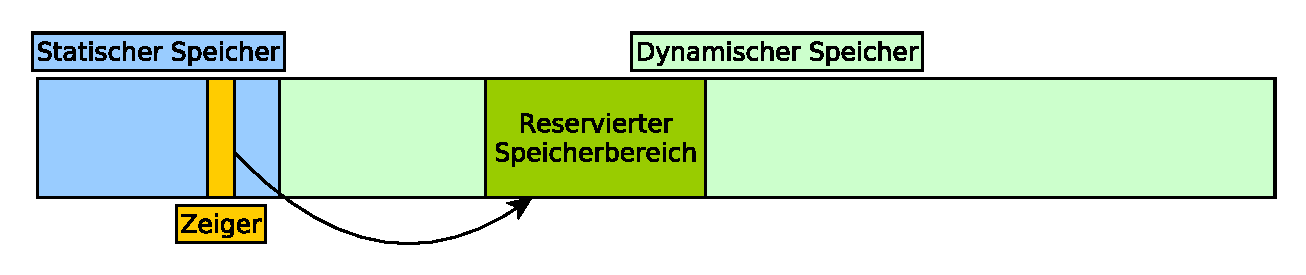
\includegraphics[width=\textwidth]{graphics/zeiger_auf_dynamischen_speicher}
\caption{\label{fig:abmem} Dynamischer und statischer Speicher eines Programms.}
\end{figure}

Bei der Benutzung von Arrays muss man immer schon zur Zeit der Übersetzung wissen, wie groß das Array maximal werden darf.
Das ist eine relativ starke Einschränkung, die sehr ineffizient sein kann.
Entweder, man hat viel zu viel Speicher bereitgestellt, oder zu wenig.
Genau passen wird es selten.

Der Speicher, der einem Programm zugeteilt ist, kann in zwei Kategorien unterteilt werden.
\begin{enumerate}
\item Statischer Speicher\\
  Dieses Teil haben wir schon kennengelernt. \index{Speicher!statisch}
  Im statischen Speicher befindet sich der Programmcode selbst, und der Speicher aller Variablen, die wir bisher deklariert haben.
  Seine Größe ist zum Zeitpunkt des Übersetzens festgelegt.

\item Dynamische Speicher\\
  Diesen Teil haben wir bisher noch nicht benutzt, aber jedes Programm kann eine bestimmte Menge an dynamischen Speicherplatz nutzen. \index{Speicher!dynamisch}
  Allerdings muss man sich zur Laufzeit des Programms selbst um das Reservieren und Freigeben dieses Speichers kümmern.
\end{enumerate}

Wenn wir also in einem Programm zum Beispiel einen Zeiger
\begin{lstlisting}
int *list;
\end{lstlisting}
deklarieren, so liegt dieser Zeiger selbst im statischen Speicherbereich.
Er kann aber auf Speicher zeigen, der im dynamischen Speicherbereich liegt.
Dies ist in Abbildung~\ref{fig:abmem} illustriert.

\subsection{Dynamische Speicherreservierung mit \texttt{malloc}}

\index{\texttt{malloc}}
Um Speicher dynamisch zu reservieren, nutzt man Funktionen aus der Standardbibliothek \verb|stdlib.h|.
Das Reservieren erledigt die Funktion \verb|malloc|, was für \emph{memory allocation} steht.
\verb|malloc| hat die folgenden Syntax:
\begin{mydefinitionblock}{Definition \texttt{malloc}}
  \begin{lstlisting}
    void *malloc(size_t size);
  \end{lstlisting}
  Reserviert Speicherzellen von der Größe \verb|size| bytes.
  \begin{itemize} 
    \itemsep0.2pt
  \item Rückgabewert: Wenn die Reservierung erfolgreich war, einen Zeiger auf den Anfang des
    reservierten Speicherbereiches, andernfalls \verb|NULL|.
  \item Eingabeparameter \verb|size|: die Größe des zu reservierenden Speicherbereiches in bytes.
  \item Beispielcode:
    \begin{lstlisting}
      int *array = (int *)malloc(sizeof(int) * 10);
    \end{lstlisting}
  \end{itemize}
  Man beachte, dass der reservierte Speicherbereich mit der Funktion \verb|free| (siehe unten) wieder freigegeben werden muss, wenn er nicht mehr benötigt wird. 
  Ansonsten steht er für das Programm nicht mehr zur Verfügung.
  Am Ende des Programms wird aller vom Programm reservierte Speicher automatisch freigegeben.
\end{mydefinitionblock}
Wir haben schon den Rückgabewert \verb|void| kennengelernt, der für keinen Rückgabewert steht.
Ein Zeiger auf \verb|void| repräsentiert einen Zeiger ohne Typ.\index{\texttt{void}}\index{Zeiger!\texttt{void}}
Er kann bzw. muss später mit einem \emph{cast} in jeden anderen Zeigertyp umgewandelt werden.
Deshalb wird im Beispielcode ein expliziter \emph{cast} nach \verb|int *| durchgeführt, den man immer bei der Benutzung von \verb|malloc| machen sollte.

Den Zeiger \verb|NULL| haben wir schon kennengelernt. \index{Zeiger!\texttt{NULL}}
\verb|malloc| gibt \verb|NULL| zurück, falls das Reservieren aus irgendeinem Grund nicht erfolgreich war.
Daher ist es sehr wichtig bei jedem Aufruf von \verb|malloc| den Rückgabewert auf \verb|NULL| zu testen!
Die Größe eines Typs in byte liefert die Funktion \verb|sizeof|.

\subsection{Speicherfreigabe mit \texttt{free}}

\index{\texttt{free}}
Wie schon angedeutet, dynamisch reservierter Speicher muss wieder freigegeben werden, wenn er nicht mehr benötigt wird.
Dafür gibt es die Funktion \verb|free|:
\begin{mydefinitionblock}{Funktion Definition \texttt{free}}
  \begin{lstlisting}
    void free(void *memory);
  \end{lstlisting}
  Gibt einen mit \verb|malloc| reservierten Speicherbereich wieder frei.
  \begin{itemize}
  \item Eingabeparameter: Zeiger auf einen Speicherbereich, der mit \verb|malloc| reserviert wurde.
  \item Beispiel:
    \begin{lstlisting}
      int *array = (int *)malloc(sizeof(int) * 10);
      free(array);
    \end{lstlisting}
  \end{itemize}
\end{mydefinitionblock}
Wendet man \verb|free| auf einen Zeiger an, der nicht auf den Anfang eines mit \verb|malloc| reservierten Bereiches zeigt, so erhält man einen Laufzeitfehler.

\subsection{Mehrdimensionale Arrays}

Bisher haben wir uns auf eindimensionale Arrays beschränkt.
Als Beispiel für ein mehrdimensionales Array betrachten wir eine Drehmatrix in zwei Dimensionen um den Winkel $\alpha$. \index{Feld!mehrdimensional}
Es handelt sich um eine lineare Abbildung, die einen zweidimensionalen Vektor $(x,y)^t$ auf den Vektor $(x',y')^t$ wie folgt abbildet:
\begin{equation}
  \left(\begin{array}{c}x^{,}\\y^{,}\end{array}\right)=
  \left(\begin{array}{cc} \cos\left(\alpha\right) & \sin\left(\alpha\right) \\
    -\sin\left(\alpha\right) & \cos\left(\alpha\right) 
  \end{array}\right)
  \left(\begin{array}{c}x\\y\end{array}\right)
\end{equation}
Die entsprechende Matrix kann man in \texttt{C} mit Hilfe von zweidimensionalen Arrays darstellen.
Die Deklaration eines statische $2\times2$ Arrays sieht wie folgt aus:
\begin{lstlisting}
double rotate2d[2][2];
\end{lstlisting}
An Hand dieser Deklaration kann man mit dem jetzigen Vorwissen ahnen, dass ein zweidimensionales Array ein Array von Arrays ist.
Daher entspricht ein solches zweidimensionales Array auch einem Zeiger auf einen Zeiger auf einen Typ.
Diskutieren wir wieder ein Beispiel:
\begin{lstlisting}
#include <math.h>
#include <stdio.h>
#include <stdlib.h>
int main()
{
  const int SPACEDIM = 2;
  const double M_PI = 3.1415;

  // Speicher reservieren
  double **array2d;
  if ((array2d = (double **)malloc(sizeof(double *) * SPACEDIM)) == NULL)
    {
      printf("Fehler in malloc\n");
      return (-1);
    }
  for (int i = 0; i < SPACEDIM; ++i)
    {
      if ((array2d[i] = (double *)malloc(sizeof(double) * SPACEDIM)) == NULL)
        {
          printf("Fehler in malloc\n");
          return (-2);
        }
    }
  // Werte zuweisen
  array2d[0][0] = cos(M_PI / 4.);
  array2d[0][1] = sin(M_PI / 4.);
  array2d[1][0] = -sin(M_PI / 4.);
  array2d[1][1] = cos(M_PI / 4.);
  // Ausgabe
  for (int i = 0; i < SPACEDIM; ++i)
    {
      for (int j = 0; j < SPACEDIM; ++j)
        {
          printf("%e ", array2d[i][j]);
        }
      printf("\n");
    }
  // Speicher freigeben
  for (int i = 0; i < SPACEDIM; ++i)
    {
      free(array2d[i]);
    }
  free(array2d);
  return (0);
}
\end{lstlisting}
\verb|array2d| ist jetzt als \verb|double**| deklariert, also als Zeiger auf einen \verb|double| Zeiger. 
Dann wird zunächst Speicher für ein Array von \verb|double*| Zeigern reserviert.
Das geschieht in Zeile $10$.
Man beachte, wie an dieser Stelle der Rückgabewert von \verb|malloc| auf \verb|NULL| getestet wird.
Eine Zuweisung der Form \verb|(x = y)| hat selbst den Wert von \verb|x|.
Anschließend wird in der Schleife, die in Zeile $14$ anfängt, für jedes Element des Arrays von \verb|double*| Zeigern selbst wieder Speicher reserviert.
Das muss nun Speicher für \verb|double| selbst sein.
Wieder testen wir den Rückgabewert von \verb|malloc| auf \verb|NULL|.

Es ist wichtig, sich klar zu machen, dass \verb|array2d| vom Typ \verb|double**| ist.
Dementsprechend zeigt es auf Elemente vom Typ \verb|double*|, die dann selbst auf Elemente vom Typ \verb|double| zeigen.
Dies ist in Abbildung~\ref{fig:mem2d} dargestellt.

\begin{figure}[!ht]
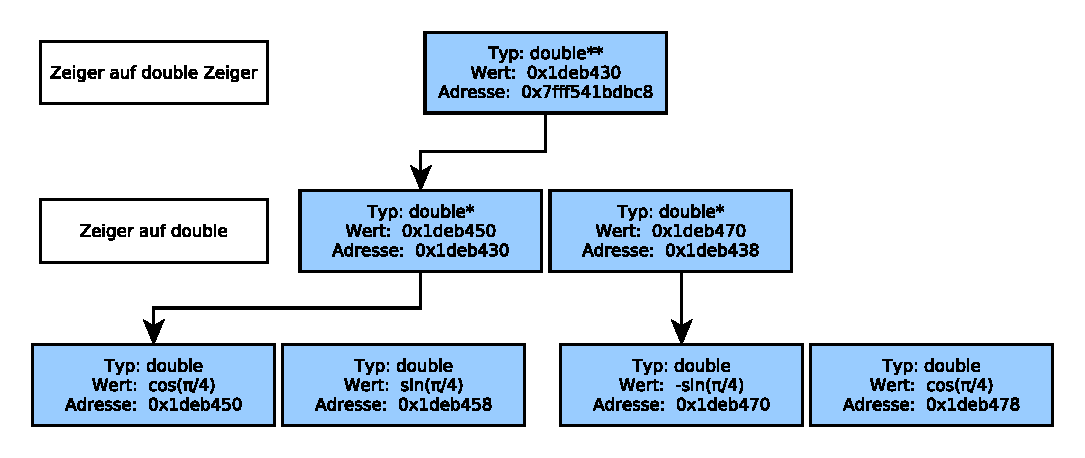
\includegraphics[width=\textwidth]{graphics/zeiger_auf_zeiger}
\caption{Illustration Zeiger auf Zeiger. \label{fig:mem2d}}
\end{figure}

Es bietet sich an für die Speicherreservierung einer zweidimensionalen Matrix eine eigene Funktion zu schreiben.
Es ist schließlich ziemlich wahrscheinlich, dass mehr als eine solche Matrix benötigt wird.
Der entsprechende Quelltext könnte beispielsweise so aussehen:
\begin{lstlisting}
#include <math.h>
#include <stdio.h>
#include <stdlib.h>

double **create2darray(const int dim)
{
  double **p1 = NULL;
  if ((p1 = (double **)malloc(sizeof(double *) * dim)) == NULL)
    {
      return (NULL);
    }
  for (int i = 0; i < dim; ++i)
    {
      if ((p1[i] = (double *)malloc(sizeof(double) * dim)) == NULL)
        {
          return (NULL);
        }
    }
  return (p1);
}

int main()
{
  const int SPACEDIM = 2;
  const double M_PI = 3.1415;

  double **array2d;
  if ((array2d = create2darray(SPACEDIM)) == NULL)
    {
      printf("Fehler in malloc\n");
      return (-1);
    }
  // Zuweisen
  array2d[0][0] = cos(M_PI / 4.);
  array2d[0][1] = sin(M_PI / 4.);
  array2d[1][0] = -sin(M_PI / 4.);
  array2d[1][1] = cos(M_PI / 4.);
  for (int i = 0; i < SPACEDIM; ++i)
    {
      for (int j = 0; j < SPACEDIM; ++j)
        {
          printf("%e ", array2d[i][j]);
        }
      printf("\n");
    }
  // hier sollte noch der Speicher freigegeben werden!
  return (0);
}
\end{lstlisting}
Die Funktion \verb|create2darray| liefert als Rückgabewert eine Variable vom Typ \verb|double**|, also genau das, was wir benötigen.
In der Funktion selbst geschieht dann das, was wir im obigen Beispiel schon gezeigt hatten.
Mit \verb|return| wird dann das Objekt zurückgegeben, für das wir Speicher reserviert haben.

An dieser Stelle sieht man einen wichtigen Unterschied zwischen der Deklaration einer Variablen und dem Reservieren von Speicher mit \verb|malloc|.
Währen beispielsweise die Variable \verb|p1| in der Funktion \verb|create2darray| natürlich nur in der Funktion selbst sichtbar ist, bleibt der mit \verb|malloc| reservierte Speicher auch außerhalb der Funktion reserviert.
Und indem wir die Adresse zu dieser Speicherstelle von der Funktion an die aufrufende Funktion übergeben, können wir den reservierten Speicherbereich auch außerhalb der Funktion nutzen.

Das bedeutet aber auch, dass Speicher, der mit \verb|malloc| reserviert wurde, und dessen Adresse wir nicht mehr kennen, nicht mehr nutzbar ist.
Auf diese Art und Weise kann man recht einfach versehentlich Programme schreiben, die den gesamten Hauptspeicher eines Rechners reservieren, ohne ihn zu nutzen.
Das führt relativ schnell zur Unbenutzbarkeit des entsprechenden Rechners.
Ein Beispiel für einen solchen Fehler ist der folgende (nicht besonders sinnvolle) Code Abschnitt
\begin{lstlisting}
int list[50];
doubke *p;
for (int i = 0; i < 50; i++)
  {
    p = malloc(sizeof(double));
    *p = i * i;
    list[i] = *p + (*p) * (*p);
  }
free(p); // falsche Stelle!
\end{lstlisting}
In jedem Durchlauf der Schleife wird Speicher für \verb|p| reserviert, ohne ihn wieder frei zu geben.
Nach Ende der Schleife ist keine der Adressen all dieser Reservierungen (bzw. nur noch die letzte) mehr verfügbar.
D.h. man kann den Speicher weder weiter benutzen, noch kann man ihn nachträglich frei geben, ein Umstand der als Speicherleck oder \emph{memory leak} bezeichnet wird.

\endinput

\newpage

\section{Komplexe Datentypen}

\subsection{Eigene Datentypen mit \texttt{typedef}}

\index{\texttt{typedef}}
Je nach Problemstellung ist es manchmal sehr hilfreich, Datenstrukturen selbst erzeugen zu können.
\texttt{C} bietet dafür die Möglichkeit, und zwar auf verschiedene Weisen.
Zunächst kann man in \texttt{C} einen neuen Typ definieren, z.B. einen eigenen Typ für reelle Zahlen:
\begin{lstlisting}
typedef float real;
\end{lstlisting}
Dieser kann im Quelltext danach wie native \texttt{C} Typen verwendet werden
\begin{lstlisting}
typedef float real;
int main()
{
  real x, y = 3.718;
  return 0;
}
\end{lstlisting}
Auf den ersten Blick mag eine eigene Definition für eine Datentyp für reelle Zahlen nicht besonders sinnvoll erscheinen.
Allerdings kann man mit dieser Typdefinition zu einem späteren Zeitpunkt sehr einfach die verwendete Genauigkeit für reelle Zahlen ändern.
Nämlich einfach, indem man die Zeile für die Typdefinition durch
\begin{lstlisting}
typedef double real;
\end{lstlisting}
ersetzt.

\subsection{Zusammengesetzte Datentypen}

\index{\texttt{struct}}
Eine weitere Art, einen neuen Datentyp zu definieren, ist zusammengesetzte Datentypen zu definieren.
Ein einfaches mathematisches Beispiel sind Vektoren, die $n$ Elemente haben.
Mithilfe des Schlüsselwrts \verb|struct| kann man in \texttt{C} zusammengesetzten Datentypen definieren, welche man sich wie Kontainer vorstellen kann.
Die allgemeine Benutzung von \verb|struct| ist wie folgt:
\begin{lstlisting}
  struct name
  {
    Type1 name1;
    Type2 name2;
    Type3 name3;
    ...
  };
\end{lstlisting}
Die Verwendung als Typ für eine Variable:
\begin{lstlisting}
  struct name variablename;
\end{lstlisting}
Als Beispiel betrachten wir einen Datentyp für kartesiche Koordinaten mit $x$, $y$ und $z$ Komponente.
Der Datentyp wird wie folgt definiert:
\begin{lstlisting}
struct coord
{
  double x, y, z;
};
\end{lstlisting}
mit drei \verb|double| Elementen, jeweils für die $x$, $y$ und $z$ Komponente.
Der Zugriff auf die einzelnen Elemente erfolgt über den Namen des \verb|struct| und den Namen des Elements, getrennt durch einen Punkt.
Für den allgemeinen Fall also wie folgt:
\begin{lstlisting}
  struct name
  {
    Type1 name1;
    Type2 name2;
    Type3 name3;
    ...
  };
  name.name1 = value;
\end{lstlisting}
In unserem Beispiel für den Koordinatentyp sieht dies wie folgt aus
\begin{lstlisting}
#include <stdio.h>

struct coord
{
  double x, y, z;
};
int main()
{
  struct coord r;
  r.x = 1.0;
  r.y = 3.4;
  r.z = -0.55;
  printf("r hat Koordinaten (%e, %e, %e)\n", r.x, r.y, r.z);
  return 0;
}
\end{lstlisting}
Also, allgemein gesprochen greift man auf die Elemente über 
\begin{lstlisting}
structname.elementname = wert;
\end{lstlisting}
zu.
Elemente können selbst wieder ein \verb|struct| sein.
Einen Unterschied gibt es beim Zugriff auf Elemente, wenn man einen Zeiger auf einen \verb|struct| benutzt.
Dort kann man direkt mit dem Pfeil Operator \verb|->| auf die Elemente zugreifen:
\begin{lstlisting}
#include <stdio.h>

struct corrd
{
  double x, y, z;
};
int main()
{
  struct coord r;
  struct coord *v = &r;
  v->x = 1.0;          // aequivalent zu (*v).x = 1.0;
  v->y = 3.4;          // aequivalent zu (*v).y = 3.4;
  v->z = -0.55         // aequivalent zu (*v).z = -0.55;
  printf("r hat Koordinaten (%e, %e, %e)\n", v->x, v->y, v->z);
  return 0;
}
\end{lstlisting}
Elemente eines \verb|struct| können natürlich auch Zeiger sein.
Allerdings muss dann Speicher außerhalb der Deklaration des \texttt{struct} reserviert werden.

\subsection{Beispiel: Datentyp für kartesische Koordinaten}

Die Verwendung von \verb|struct| ist sehr hilfreich, um logisch zusammengehörige Daten gesammelt zu übergeben und zu bearbeiten.
Es muss dann nicht mehr jedes Element einzeln übergeben werden, sondern nur noch einmal der Kontainer.
Der Zusammenhang der einzelnen Elemente bleibt damit erhalten.
Man könnte nun beispielsweise eine Funktion für die Quadratnorm einer Koordinate wie folgt schreiben:
\begin{lstlisting}
#include <stdio.h>

struct coord
{
  double x, y, z;
};
double sqnorm(struct coord r) {
  return(r.x*r.x + r.y*r.y + r.z*r.z);
}

int main()
{
  struct coord r;
  r.x = 1.0;
  r.y = 3.4;
  r.z = -0.55;
  printf("r hat Quadratnorm %e\n'', sqnorm(r));
  return 0;
}
\end{lstlisting}
Mit einem \verb|struct| wird ebenfalls einer neuer Typ bereitgestellt.
Der entsprechende Name enthält aber immer das Schlüsselwort \verb|struct|, in unserem Fall \verb|struct coord|. 
Man kann einen \verb|struct| mit einem \verb|typedef| kombinieren, um nicht immer \verb|struct| schreiben zu müssen.
Im Quelltext sähe das so aus:
\begin{lstlisting}
struct coord
{
  double x, y, z;
};
typedef struct coord coord;
\end{lstlisting}
Das sieht etwas verwirrend aus, weil \verb|coord| zweimal auftaucht.
Aber der Ausdruck wird klar, wenn man sich erinnert, dass \verb|struct coord| im Prinzip ein Typ ist.
Und damit ist der Name \verb|coord| noch nicht vergeben.
Die etwas gebräuchlichere Art obiger Typdefinition geht über die Möglichekeit eines anonymen \verb|struct|.
Man kann nämlich auch schreiben:
\begin{lstlisting}
typedef struct
{
  double x, y, z;
} coord;
\end{lstlisting}
Damit ist natürlich \verb|struct coord| nicht definiert, aber man kann \verb|coord| wie einen \texttt{C} Typ verwenden.


\endinput



%\input{stapelspeicher}
%\input{endprojekt}


\printindex

\end{document}
